% Generated fragments require trusted human review before compilation.
% This binder never requests shell escape or runs external tools.
\documentclass[11pt]{article}
% Trusted shared apparatus. Requires LuaLaTeX; never use shell escape.
\usepackage{fontspec}
\defaultfontfeatures{Ligatures=TeX}
\IfFontExistsTF{Noto Serif}{\setmainfont{Noto Serif}}{%
  \IfFontExistsTF{DejaVu Serif}{\setmainfont{DejaVu Serif}}{%
    \IfFontExistsTF{Times New Roman}{\setmainfont{Times New Roman}}{%
      \PackageError{gelfand-binder}{No configured Cyrillic serif font installed}{Install Noto Serif or DejaVu Serif, or select an installed Cyrillic font.}%
    }%
  }%
}
\IfFontExistsTF{Noto Sans}{\setsansfont{Noto Sans}}{%
  \IfFontExistsTF{DejaVu Sans}{\setsansfont{DejaVu Sans}}{\setsansfont{Arial}}%
}
\IfFontExistsTF{Noto Sans Mono}{\setmonofont{Noto Sans Mono}}{%
  \IfFontExistsTF{DejaVu Sans Mono}{\setmonofont{DejaVu Sans Mono}}{\setmonofont{Courier New}}%
}
\usepackage[a4paper,margin=22mm]{geometry}
\usepackage{amsmath,amssymb,amsthm,mathtools}
\usepackage{xcolor}
\usepackage{tikz}
\usepackage{tikz-cd}
\usetikzlibrary{arrows.meta,positioning,calc}
\usepackage{hyperref}
\hypersetup{unicode=true,colorlinks=true,linkcolor=blue,pdftitle={Gelfand transcription binder}}
\newtheorem{theorem}{Theorem}
\newtheorem{lemma}{Lemma}
\newtheorem{proposition}{Proposition}
\newtheorem{corollary}{Corollary}
\theoremstyle{definition}
\newtheorem{definition}{Definition}
\newtheorem{example}{Example}
\theoremstyle{remark}
\newtheorem{remark}{Remark}
\setlength{\parindent}{0pt}
\setlength{\parskip}{0.55em}
\setlength{\emergencystretch}{3em}
\newcommand{\SourcePage}[2]{%
  \clearpage\phantomsection\label{#1:source-page}%
  \addcontentsline{toc}{subsection}{#1}%
  {\small\sffamily\color{blue!60!black}Source scan frame: #1; visible page/leaf label: #2}\par\medskip%
}
\newcommand{\Unclear}[3]{%
  \begingroup\color{orange!70!black}%
  [Unresolved reading #1/#2: #3]\endgroup%
}
\newcommand{\Incomplete}[3]{%
  \par\begingroup\color{red!65!black}\textbf{Incomplete #1/#2:} #3\endgroup\par%
}
\newcommand{\SourceFigure}[3]{%
  \par\begingroup\color{blue!60!black}\textbf{\hyperref[#1:source-page]{Source figure #1/#2}:} #3%
  \par\textit{Consult the authoritative scan at this locator.}\endgroup\par%
}



% Reader layout only. Original diplomatic text is retained verbatim.
\setlength{\parskip}{0.35em}
\setlength{\emergencystretch}{4em}
\renewcommand{\SourcePage}[2]{%
  \par\addvspace{1em}\phantomsection\label{#1:source-page}%
  \addcontentsline{toc}{subsection}{#1}%
  {\footnotesize\sffamily\color{blue!55!black}#1%
    \def\givenlabel{#2}\def\nolabel{unlabelled}%
    \ifx\givenlabel\nolabel\else\quad[номер в источнике: #2]\fi
  }\par\nobreak\smallskip%
}
\renewcommand{\Unclear}[3]{%
  \begingroup\color{orange!65!black}%
  \ifmmode\text{[неясно: #3]}\else[неясно: #3]\fi\endgroup%
}
\renewcommand{\Incomplete}[3]{%
  \par\begingroup\color{red!60!black}\textbf{Неразобранный фрагмент:} #3%
  \endgroup\par%
}
\renewcommand{\SourceFigure}[3]{%
  \par\begingroup\color{blue!55!black}\textbf{Рисунок:} #3%
  \par{\small\textit{Исходный рисунок: \hyperref[#1:source-page]{#1}, #2.}}%
  \endgroup\par%
}
\hypersetup{pdftitle={Семинар И. М. Гельфанда. Дипломатическая транскрипция},pdfauthor={},pdfsubject={Русское рабочее издание с отмеченными сомнительными чтениями}}

\usepackage[normalem]{ulem}
\usepackage{newunicodechar}
\usepackage{adjustbox}
\newfontfamily\SourceSymbolFont{Segoe UI Symbol}
\newfontfamily\SourceCJKFont{MS Gothic}
\let\DiplomaticMathUnderline\underline
\renewcommand{\underline}[1]{\ifmmode\DiplomaticMathUnderline{#1}\else\uline{#1}\fi}
\newunicodechar{→}{\ifmmode\text{{\SourceSymbolFont\char"2192}}\else{\SourceSymbolFont\char"2192}\fi}
\newunicodechar{⇒}{\ifmmode\text{{\SourceSymbolFont\char"21D2}}\else{\SourceSymbolFont\char"21D2}\fi}
\newunicodechar{∀}{\ifmmode\text{{\SourceSymbolFont\char"2200}}\else{\SourceSymbolFont\char"2200}\fi}
\newunicodechar{∂}{\ifmmode\text{{\SourceSymbolFont\char"2202}}\else{\SourceSymbolFont\char"2202}\fi}
\newunicodechar{∈}{\ifmmode\text{{\SourceSymbolFont\char"2208}}\else{\SourceSymbolFont\char"2208}\fi}
\newunicodechar{∌}{\ifmmode\text{{\SourceSymbolFont\char"220C}}\else{\SourceSymbolFont\char"220C}\fi}
\newunicodechar{√}{\ifmmode\text{{\SourceSymbolFont\char"221A}}\else{\SourceSymbolFont\char"221A}\fi}
\newunicodechar{∞}{\ifmmode\text{{\SourceSymbolFont\char"221E}}\else{\SourceSymbolFont\char"221E}\fi}
\newunicodechar{∧}{\ifmmode\text{{\SourceSymbolFont\char"2227}}\else{\SourceSymbolFont\char"2227}\fi}
\newunicodechar{∩}{\ifmmode\text{{\SourceSymbolFont\char"2229}}\else{\SourceSymbolFont\char"2229}\fi}
\newunicodechar{∪}{\ifmmode\text{{\SourceSymbolFont\char"222A}}\else{\SourceSymbolFont\char"222A}\fi}
\newunicodechar{∫}{\ifmmode\text{{\SourceSymbolFont\char"222B}}\else{\SourceSymbolFont\char"222B}\fi}
\newunicodechar{∴}{\ifmmode\text{{\SourceSymbolFont\char"2234}}\else{\SourceSymbolFont\char"2234}\fi}
\newunicodechar{∼}{\ifmmode\text{{\SourceSymbolFont\char"223C}}\else{\SourceSymbolFont\char"223C}\fi}
\newunicodechar{≈}{\ifmmode\text{{\SourceSymbolFont\char"2248}}\else{\SourceSymbolFont\char"2248}\fi}
\newunicodechar{≠}{\ifmmode\text{{\SourceSymbolFont\char"2260}}\else{\SourceSymbolFont\char"2260}\fi}
\newunicodechar{≤}{\ifmmode\text{{\SourceSymbolFont\char"2264}}\else{\SourceSymbolFont\char"2264}\fi}
\newunicodechar{≥}{\ifmmode\text{{\SourceSymbolFont\char"2265}}\else{\SourceSymbolFont\char"2265}\fi}
\newunicodechar{⊕}{\ifmmode\text{{\SourceSymbolFont\char"2295}}\else{\SourceSymbolFont\char"2295}\fi}
\newunicodechar{⊗}{\ifmmode\text{{\SourceSymbolFont\char"2297}}\else{\SourceSymbolFont\char"2297}\fi}
\newunicodechar{①}{\ifmmode\text{{\SourceSymbolFont\char"2460}}\else{\SourceSymbolFont\char"2460}\fi}
\newunicodechar{②}{\ifmmode\text{{\SourceSymbolFont\char"2461}}\else{\SourceSymbolFont\char"2461}\fi}
\newunicodechar{③}{\ifmmode\text{{\SourceSymbolFont\char"2462}}\else{\SourceSymbolFont\char"2462}\fi}
\newunicodechar{④}{\ifmmode\text{{\SourceSymbolFont\char"2463}}\else{\SourceSymbolFont\char"2463}\fi}
\newunicodechar{Ⓗ}{\ifmmode\text{{\SourceSymbolFont\char"24BD}}\else{\SourceSymbolFont\char"24BD}\fi}
\newunicodechar{〃}{\ifmmode\text{{\SourceCJKFont\char"3003}}\else{\SourceCJKFont\char"3003}\fi}


% Reader revision 3. Annotation wording and candidates remain unchanged.
\usetikzlibrary{shapes.geometric,decorations.pathreplacing,decorations.markings,patterns,fit}
\newsavebox{\ReaderAnnotationBox}
\newcommand{\ReaderAnnotation}[1]{%
  \sbox{\ReaderAnnotationBox}{[неясно: #1]}%
  \ifdim\wd\ReaderAnnotationBox>.70\linewidth
    \parbox[t]{.70\linewidth}{\raggedright[неясно: #1]}%
  \else\usebox{\ReaderAnnotationBox}\fi%
}
\ExplSyntaxOn
\cs_new_protected:Npn \reader_unclear_candidate:n #1
 {
  \tl_set:Nx \l_tmpa_tl { \tl_to_str:n {#1} }
  % Text explicitly guarded inside a mathematical candidate remains math-safe.
  \regex_replace_all:nnN { \\(?:text|textrm|textnormal|textbf|operatorname)\s*\{[^{}]*\} } { } \l_tmpa_tl
  \regex_match:nVTF { [\x{0400}-\x{052F}] | \$ } \l_tmpa_tl
   { \ifmmode \text{\ReaderAnnotation{#1}} \else \ReaderAnnotation{#1} \fi }
   {
    \ifmmode
      [\text{неясно:~}#1]
    \else
      \regex_match:nVTF { [_^] | \\ } \l_tmpa_tl
       { \ensuremath{[\text{неясно:~}#1]} }
       { \ReaderAnnotation{#1} }
    \fi
   }
 }
\RenewDocumentCommand \Unclear { m m m }
 { \begingroup\color{orange!65!black}\reader_unclear_candidate:n{#3}\endgroup }
\ExplSyntaxOff
\newsavebox{\ReaderIncompleteBox}
\newcommand{\ReaderIncompleteNote}[1]{%
 \sbox{\ReaderIncompleteBox}{\textbf{Неразобранный фрагмент:} #1}%
 \ifdim\wd\ReaderIncompleteBox>.70\linewidth
  \parbox[t]{.70\linewidth}{\raggedright\textbf{Неразобранный фрагмент:} #1}%
 \else\usebox{\ReaderIncompleteBox}\fi%
}
\renewcommand{\Incomplete}[3]{%
 \ifmmode\text{\color{red!60!black}\ReaderIncompleteNote{#3}}%
 \else\par\begingroup\color{red!60!black}\textbf{Неразобранный фрагмент:} #3\endgroup\par\fi%
}
% Ragged right avoids stretching long untranslated abbreviations into margins.
\AtBeginDocument{\raggedright}
\newunicodechar{А}{\ifmmode\text{\char"410\relax}\else\char"410\relax\fi}
\newunicodechar{Б}{\ifmmode\text{\char"411\relax}\else\char"411\relax\fi}
\newunicodechar{В}{\ifmmode\text{\char"412\relax}\else\char"412\relax\fi}
\newunicodechar{Г}{\ifmmode\text{\char"413\relax}\else\char"413\relax\fi}
\newunicodechar{Д}{\ifmmode\text{\char"414\relax}\else\char"414\relax\fi}
\newunicodechar{Е}{\ifmmode\text{\char"415\relax}\else\char"415\relax\fi}
\newunicodechar{Ж}{\ifmmode\text{\char"416\relax}\else\char"416\relax\fi}
\newunicodechar{З}{\ifmmode\text{\char"417\relax}\else\char"417\relax\fi}
\newunicodechar{И}{\ifmmode\text{\char"418\relax}\else\char"418\relax\fi}
\newunicodechar{Й}{\ifmmode\text{\char"419\relax}\else\char"419\relax\fi}
\newunicodechar{К}{\ifmmode\text{\char"41A\relax}\else\char"41A\relax\fi}
\newunicodechar{Л}{\ifmmode\text{\char"41B\relax}\else\char"41B\relax\fi}
\newunicodechar{М}{\ifmmode\text{\char"41C\relax}\else\char"41C\relax\fi}
\newunicodechar{Н}{\ifmmode\text{\char"41D\relax}\else\char"41D\relax\fi}
\newunicodechar{О}{\ifmmode\text{\char"41E\relax}\else\char"41E\relax\fi}
\newunicodechar{П}{\ifmmode\text{\char"41F\relax}\else\char"41F\relax\fi}
\newunicodechar{Р}{\ifmmode\text{\char"420\relax}\else\char"420\relax\fi}
\newunicodechar{С}{\ifmmode\text{\char"421\relax}\else\char"421\relax\fi}
\newunicodechar{Т}{\ifmmode\text{\char"422\relax}\else\char"422\relax\fi}
\newunicodechar{У}{\ifmmode\text{\char"423\relax}\else\char"423\relax\fi}
\newunicodechar{Ф}{\ifmmode\text{\char"424\relax}\else\char"424\relax\fi}
\newunicodechar{Х}{\ifmmode\text{\char"425\relax}\else\char"425\relax\fi}
\newunicodechar{Ц}{\ifmmode\text{\char"426\relax}\else\char"426\relax\fi}
\newunicodechar{Ч}{\ifmmode\text{\char"427\relax}\else\char"427\relax\fi}
\newunicodechar{Ш}{\ifmmode\text{\char"428\relax}\else\char"428\relax\fi}
\newunicodechar{Щ}{\ifmmode\text{\char"429\relax}\else\char"429\relax\fi}
\newunicodechar{Ъ}{\ifmmode\text{\char"42A\relax}\else\char"42A\relax\fi}
\newunicodechar{Ы}{\ifmmode\text{\char"42B\relax}\else\char"42B\relax\fi}
\newunicodechar{Ь}{\ifmmode\text{\char"42C\relax}\else\char"42C\relax\fi}
\newunicodechar{Э}{\ifmmode\text{\char"42D\relax}\else\char"42D\relax\fi}
\newunicodechar{Ю}{\ifmmode\text{\char"42E\relax}\else\char"42E\relax\fi}
\newunicodechar{Я}{\ifmmode\text{\char"42F\relax}\else\char"42F\relax\fi}
\newunicodechar{а}{\ifmmode\text{\char"430\relax}\else\char"430\relax\fi}
\newunicodechar{б}{\ifmmode\text{\char"431\relax}\else\char"431\relax\fi}
\newunicodechar{в}{\ifmmode\text{\char"432\relax}\else\char"432\relax\fi}
\newunicodechar{г}{\ifmmode\text{\char"433\relax}\else\char"433\relax\fi}
\newunicodechar{д}{\ifmmode\text{\char"434\relax}\else\char"434\relax\fi}
\newunicodechar{е}{\ifmmode\text{\char"435\relax}\else\char"435\relax\fi}
\newunicodechar{ж}{\ifmmode\text{\char"436\relax}\else\char"436\relax\fi}
\newunicodechar{з}{\ifmmode\text{\char"437\relax}\else\char"437\relax\fi}
\newunicodechar{и}{\ifmmode\text{\char"438\relax}\else\char"438\relax\fi}
\newunicodechar{й}{\ifmmode\text{\char"439\relax}\else\char"439\relax\fi}
\newunicodechar{к}{\ifmmode\text{\char"43A\relax}\else\char"43A\relax\fi}
\newunicodechar{л}{\ifmmode\text{\char"43B\relax}\else\char"43B\relax\fi}
\newunicodechar{м}{\ifmmode\text{\char"43C\relax}\else\char"43C\relax\fi}
\newunicodechar{н}{\ifmmode\text{\char"43D\relax}\else\char"43D\relax\fi}
\newunicodechar{о}{\ifmmode\text{\char"43E\relax}\else\char"43E\relax\fi}
\newunicodechar{п}{\ifmmode\text{\char"43F\relax}\else\char"43F\relax\fi}
\newunicodechar{р}{\ifmmode\text{\char"440\relax}\else\char"440\relax\fi}
\newunicodechar{с}{\ifmmode\text{\char"441\relax}\else\char"441\relax\fi}
\newunicodechar{т}{\ifmmode\text{\char"442\relax}\else\char"442\relax\fi}
\newunicodechar{у}{\ifmmode\text{\char"443\relax}\else\char"443\relax\fi}
\newunicodechar{ф}{\ifmmode\text{\char"444\relax}\else\char"444\relax\fi}
\newunicodechar{х}{\ifmmode\text{\char"445\relax}\else\char"445\relax\fi}
\newunicodechar{ц}{\ifmmode\text{\char"446\relax}\else\char"446\relax\fi}
\newunicodechar{ч}{\ifmmode\text{\char"447\relax}\else\char"447\relax\fi}
\newunicodechar{ш}{\ifmmode\text{\char"448\relax}\else\char"448\relax\fi}
\newunicodechar{щ}{\ifmmode\text{\char"449\relax}\else\char"449\relax\fi}
\newunicodechar{ъ}{\ifmmode\text{\char"44A\relax}\else\char"44A\relax\fi}
\newunicodechar{ы}{\ifmmode\text{\char"44B\relax}\else\char"44B\relax\fi}
\newunicodechar{ь}{\ifmmode\text{\char"44C\relax}\else\char"44C\relax\fi}
\newunicodechar{э}{\ifmmode\text{\char"44D\relax}\else\char"44D\relax\fi}
\newunicodechar{ю}{\ifmmode\text{\char"44E\relax}\else\char"44E\relax\fi}
\newunicodechar{я}{\ifmmode\text{\char"44F\relax}\else\char"44F\relax\fi}
\newunicodechar{Ё}{\ifmmode\text{\char"401\relax}\else\char"401\relax\fi}
\newunicodechar{ё}{\ifmmode\text{\char"451\relax}\else\char"451\relax\fi}


% Reader-only pairing support; accepted raw bodies remain unchanged.
\RequirePackage{graphicx}
\RequirePackage{adjustbox}
\newcommand{\ReaderOriginalPanel}[2]{%
  \begin{minipage}[t]{.48\linewidth}\vspace{0pt}\centering
    \includegraphics[width=\linewidth,keepaspectratio]{#1}\par\smallskip
    {\scriptsize Оригинал рукописного рисунка: #2}\par
  \end{minipage}%
}
\newcommand{\ReaderDiagramPair}[3]{%
  \par\noindent\begingroup
  \ReaderOriginalPanel{#1}{#2}\hfill
  \begin{minipage}[t]{.48\linewidth}\vspace{0pt}\centering
    {\scriptsize Типографское воссоздание}\par\smallskip
    \begin{adjustbox}{max width=\linewidth}#3\end{adjustbox}\par
  \end{minipage}%
  \endgroup\par\smallskip
}
\newcommand{\ReaderDescriptionPair}[3]{%
  \par\noindent\begingroup
  \ReaderOriginalPanel{#1}{#2}\hfill
  \begin{minipage}[t]{.48\linewidth}\vspace{0pt}\raggedright
    {\scriptsize Типографское описание}\par\smallskip
    #3\par
  \end{minipage}%
  \endgroup\par\smallskip
}


\begin{document}
\begin{center}
{\Large Семинар И. М. Гельфанда}\par\medskip
{\LARGE Дипломатическая транскрипция}\par\bigskip
{\large Рабочее русское издание}\par\medskip
{\large Том 12 из 34. Архивная глава 012}\par\bigskip
Кадры GELFAND-P000738 -- GELFAND-P000776\par
\end{center}
\medskip
Сокращения, отменённые записи и сомнительные чтения сохранены.
Неразобранные фрагменты отмечены в тексте. Математические утверждения
источника переданы без молчаливых исправлений.

В текущем комплекте приняты 165 из 165 возвратов; учтены 1527 из 1527 кадров. Кадров без принятого возврата: 0.
Статусы кадров в отчётах о полноте: транскрибированы 1168, неразборчивы 357, частично прочитаны 1, недоступны 1.
Нерешённых записей журнала чтений: 6820.
Статус «неразборчивый» может отмечать локальную утрату зачёркнутой записи;
он не означает отсутствия всего кадра.
Сверка с рукописью продолжается. Рабочие журналы чтений и происхождения
данных сохранены отдельно.

Ограничения исходного комплекта: повреждённый исходный скан GELFAND-P000722; каталожные записи 603, 694 без сканов; в архивной главе 029 не перечислена часть 25.

Границы кадров показаны небольшими синими указателями; печатный текст
продолжается без обязательного разрыва страницы после каждого кадра.
\bigskip\hrule\bigskip
\SourcePage{GELFAND-P000738}{6}
% Координаты областей далее даны в пикселях оригинала (x1,y1,x2,y2), начало слева сверху.
% Оригинал 2417 x 3473 просмотрен целиком; заголовок (250,75,1350,402) проверен при увеличении 3x.
\underline{\underline{21/$\overline{\underline{\mathrm{XI}}}$-77.}}\qquad
\underline{\underline{Сем. Гельфанда.}}

\underline{\textbf{Ю. И. Манин.}}
[На скане имя заключено в красную прямоугольную рамку.]

(о работе с \underline{В. Дринфельдом})

\underline{Описание автодуальных решений ур-й Янга-Миллса}

\begin{equation*}
\mathbb{R}^{4}\ni(x_1,x_2,x_3,x_4).
\end{equation*}
Неизвестные функции:
\begin{equation*}
A_\mu(x)\in u(r),\qquad r\geq 2
\end{equation*}
% Пояснения к u(r): (620,625,2417,824), увеличение 3x.
(эрмитовы или антиэрмитовы матрицы; в алгебре Ли)

[Под $u(r)$ скобка и стрелка от пояснения:]
алгебра Ли $U(r)$, $u(r)$ --- множество косоэрмитовых $r\times r$ матриц.

% Формулы (1), (2): (155,742,1530,1405), увеличение 3x; правая часть пояснения к (2) проверена по оригиналу.
\begin{equation*}
F_{\mu\nu}(x)\underset{\mathrm{def}}{=}
\frac{\partial}{\partial x_\mu}A_\nu
-\frac{\partial}{\partial x_\nu}A_\mu
+[A_\mu,A_\nu]
\tag{1}
\end{equation*}

1) \underline{Уравнения дуальности:}

$\rho\sigma$ --- доп. пара индексов к $\mu\nu$;
$F_{\mu\nu}=\pm F_{\rho\sigma}$; точнее:
\begin{equation*}
F_{\mu\nu}=\varepsilon^{\mu\nu\rho\sigma}F_{\rho\sigma}
\tag{2}
\end{equation*}
($\varepsilon^{\mu\nu\rho\sigma}$ --- знак перестановки).

2) \underline{Условия регулярности:} А) в конечн. точках Б) в бесконечности

% Текст перед (3): (190,1510,2417,1795), увеличение 3x.
А) особенности могут быть в конечных точках сняты калибровкой.

Точнее, рассм. расслоение $\mathbb{C}^{r}\times\mathbb{R}^{4}$ и в нем базис сечений;
ковариантн. диффер., определяемое матрицами $A_\mu$, задается формулой:

% Формула (3): (390,1800,1830,2053), увеличение 5x.
\begin{equation*}
\partial_\mu
\begin{pmatrix}s_1\\ \vdots\\ s_r\end{pmatrix}
=A_\mu\begin{pmatrix}s_1\\ \vdots\\ s_r\end{pmatrix},
\qquad
\partial_\mu s_i=\sum_{i=1}^{r}A_\mu^{ij}s_j.
\tag{3}
\end{equation*}
\Unclear{GELFAND-P000738}{eq-03-summation}{[В нижнем пределе суммы написано $i=1$; индекс у $s_i$ обведен.]}
[Стрелка к первому столбцу: базисные сечения $s_1,\ldots,s_r$.]

% Смена базиса: (210,2035,2417,2247), увеличение 3x.
Перейдем к другому базису. Получим преобразование (калибровочное преобразование):
\begin{equation*}
A_\mu\mapsto u^{-1}\partial_\mu u+u^{-1}A_\mu u=A'_\mu
\tag{4}
\end{equation*}

\underline{Условие регулярности в конечной точке:} имеется настоящая
связность без особенностей, т. е. особ. $A_\mu$ можно ликвидировать калибровкой.

Переход:
\begin{equation*}
\begin{pmatrix}s_1\\ \vdots\\ s_r\end{pmatrix}
\mapsto u\begin{pmatrix}s_1\\ \vdots\\ s_r\end{pmatrix}
\end{equation*}
[К $u$ снизу направлена стрелка с подписью $r\times r$.]

% Нижняя часть: (170,2830,2417,3473), увеличение 3x; P=∞: (655,2840,900,2925), 8x.
Б) \underline{Условия в $P=\infty$.}

Расслоение на $\mathbb{R}^{4}$ продолжается до рассл. над
$S^{4}=\mathbb{R}^{4}\cup\{\infty\}$.

\begin{center}
\begin{adjustbox}{max width=\linewidth}
\begin{tikzcd}[row sep=small]
L\arrow[d,"\mathbb{C}^{r}"]\\
S^{4}
\end{tikzcd}
\end{adjustbox}
\qquad $L$ --- пр-во нашего расслоения.
\end{center}

\underline{Усл. регулярности:} Связность $\partial_\mu$ продолжается до связности в $L$ над $S^{4}$
(расслоение $L$ уже не обязательно тривиально)

\SourcePage{GELFAND-P000739}{unlabelled}
% Оригинал 2416 x 3472 просмотрен целиком. Координаты в пикселях оригинала, начало слева сверху.
% Верхние строки: (200,70,2220,450), увеличение 3x.
Это тоже означает, что на бесконечности подкруткой можно
ликвидировать особенность.

Существенный инвариант решения --- расслоение $L$. Это дискретный
инвариант. На $L$ структура унитарного расслоения.

\underline{Классификация $L$.}

Склейка тривиализаций на экваторе есть отображение $S^{3}\to U(r)$,
т. е. элемент $\pi_3(U(r))=\mathbb{Z}$.

% Пояснение и вложение: (210,690,2350,1040), 3x; слово «дискретный»: (1400,680,2350,776), 5x.
($SU(2)\subset U(r)$, $SU(2)\cong S^{3}$; отсюда целочисленный дискретный
инвариант = степень отображения $n$ = число Понтрягина)

вложение $SU(2)\subset U(r)$ берется вида
\begin{center}
\begin{adjustbox}{max width=\linewidth}
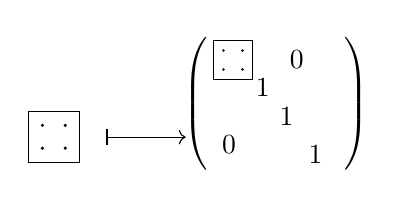
\begin{tikzpicture}[x=1cm,y=1cm]
\draw (0,0) rectangle (0.65,0.65);
\fill (0.18,0.47) circle (0.022);
\fill (0.47,0.47) circle (0.022);
\fill (0.18,0.18) circle (0.022);
\fill (0.47,0.18) circle (0.022);
\draw[->] (1,0.32) -- (2,0.32);
\draw (1,0.22) -- (1,0.42);
\node at (2.15,0.75) {$\left(\vphantom{\begin{matrix}1\\1\\1\\1\end{matrix}}\right.$};
\node at (4.15,0.75) {$\left.\vphantom{\begin{matrix}1\\1\\1\\1\end{matrix}}\right)$};
\draw (2.35,1.05) rectangle (2.85,1.55);
\fill (2.48,1.42) circle (0.018);
\fill (2.72,1.42) circle (0.018);
\fill (2.48,1.18) circle (0.018);
\fill (2.72,1.18) circle (0.018);
\node at (2.98,0.95) {$1$};
\node at (3.28,0.58) {$1$};
\node at (3.65,0.1) {$1$};
\node at (3.41,1.31) {$0$};
\node at (2.55,0.22) {$0$};
\end{tikzpicture}
\end{adjustbox}
\end{center}

\underline{Будем считать} $n\geq 0$ и дуальные условия

% Extra source closing parenthesis after (2) confirmed at bbox (1600,1170,1830,1345), 8x.
($n<0\ \Rightarrow$ можно изменить знак в ур-и (2))
--- антидуальные реш. --- свести к $n>0$)

\underline{План дальнейшего:}

% Зачеркнутая строка: (285,1438,1010,1530), увеличение 5x.
\Incomplete{GELFAND-P000739}{plan-deleted-line}{[Под заголовком зачеркнута целая строка; текст под плотной штриховкой не восстановлен.]}

% Схема: (130,1410,1710,2110), увеличение 3x. Зачеркнутая подпись: (1000,1748,1370,1830), 6x.
\SourceFigure{GELFAND-P000739}{diagram-plan}{Слева в круглых скобках изображены $L\downarrow S^{4}$ и, через запятую, $A_\mu$. От них волнистая стрелка идет вправо к большой левой квадратной скобке. Вверху внутри скобки $H\times S^{4}\downarrow S^{4}$; к $H$ сверху слева направлена стрелка от $2n+r$. Справа написано $H=\mathbb{C}^{2n+r}$. Ниже внутри скобки: «Здесь:», зачеркнутая подпись, «эрмитова метрика», «тривиальная связность». Из нижней части скобки диагональная стрелка направлена вверх влево к исходной паре. К этой стрелке снизу слева направлена другая стрелка от подписи «Явн. конструируемое разл. на ортог. части». Требует проверки зачеркнутая подпись внутри скобки; она отдельно отмечена ниже.}
\Incomplete{GELFAND-P000739}{diagram-deleted-caption}{[После «Здесь:» зачеркнуто короткое словосочетание; различима начальная «с», остальная подпись не восстановлена.]}

\begin{equation*}
\begin{array}{lccccc}
\text{Размерности:}&2n+r&&r&&2n\\
&\downarrow&&\downarrow&&\downarrow\\
\text{Разложение:}&H\times S^{4}&=&L&\oplus&L^{\perp}
\end{array}
\end{equation*}

% Текст о связности: (455,2125,2120,2340), увеличение 3x.
$\{A_\mu\}$ --- прямое слагаемое тривиальной связности в $H\times S^{4}$

(Дифференцируем и проектируем на $L$).

Унитарность связности доказывается.

% Примечание в квадратных скобках: (210,2350,2300,2730), 3x; «риманово м-во»: (1050,2420,1750,2540), 5x.
[Это обобщение того, что риманово м-во можно вложить в
евклидово; можно ли [вставлено над строкой: всегда] вложить расслоение со связностью?]

Какие разложения приводят к автодуальным полям?

Надо от базы $S^{4}$ перейти к ее \underline{комплексификации}.

% Нижние формулы и текст: (245,2840,2060,3350), увеличение 3x.
В $\mathbb{C}^{4}$ рассмотрим отобр.
\begin{equation*}
\sigma:\ z\mapsto(-\overline{z}_2,\overline{z}_1,-\overline{z}_4,\overline{z}_3).
\end{equation*}
[От $\mathbb{C}^{4}$ стрелка вниз к подписи:]
$z=(z_1,z_2,z_3,z_4)$

(в кватернионах умножение на $i$)

У $\sigma$ нет неподв. точек (кроме $0$) и неподв. прямых, а есть
инвар. плоскости
\begin{equation*}
\mathbb{C}z+\mathbb{C}\sigma(z)\subset\mathbb{C}^{4}
\tag{5}
\end{equation*}

\SourcePage{GELFAND-P000740}{7}
% Reviewed full-resolution original 2416x3472; text crops at 3x.
% review top bbox=(100,0,2370,540), scale=3.
Будем называть их \underline{вещественными} (или \underline{$\sigma$-инвариантными})
($\sigma$ — инволюция).

\begin{equation*}
\{\sigma\text{-инвар. плоскости}\}=S^4 \tag{6}
\end{equation*}
(\underline{док-во опускается})

(в $\mathbb{C}P^3$ это мн-во $\sigma$-инвар. прямых).

% review compactification-cancel bbox=(710,505,827,620), scales=3,10; U200.
$E^4\subset$ [зачёркнуто: \Unclear{GELFAND-P000740}{compactification-cancel}{неразборчивый знак}]
$S^4=E^4\cup\{\infty\}$.

% review map bbox=(180,495,2250,1200), scale=3.
Отсюда есть отображение
\begin{equation*}
\mathbb{C}^4\setminus\{0\}\overset{D}{\longrightarrow}S^4\supset E^4. \tag{7}
\end{equation*}
\begin{equation*}
z\longmapsto \sigma\text{-инвар. плоск., прох. через }z.
\end{equation*}
Напишем $D$ в координатах (в $E^4$ координаты $(x_i)$).
Нормировка как у Захарова-Белавина.

% review coordinates bbox=(250,1140,1800,1645), scale=3.
\begin{equation*}
(z_1,z_2,z_3,z_4)\longmapsto
\begin{cases}
x_2+i x_1=\dfrac{z_1\bar z_3+\bar z_2z_4}{|z_3|^2+|z_4|^2},\\[6pt]
x_4+i x_3=\dfrac{\bar z_2z_3-z_1\bar z_4}{|z_3|^2+|z_4|^2}.
\end{cases}
\end{equation*}
(плюккеровы координаты [вставлено: $\sigma$-инв.] плоскости, проходящей через т. $z$)

Это отображение
\begin{equation*}
\mathbb{C}^4\setminus\{z_3=z_4=0\}\longrightarrow E^4.
\end{equation*}
\underline{Замечание:} для восстан. $\sigma$-инв. пл. достаточно 3-х координат.

% review lemma bbox=(210,1730,2270,2230), scale=3.
% review names bbox=(1020,1925,1945,2055), scale=5.
% review attribution-numeral bbox=(635,1885,938,2050), scales=3,10; U201.
\underline{\underline{Лемма 1}}
(АУБЗ [над буквами соответственно: $4$, $2$,
\Unclear{GELFAND-P000740}{attribution-numeral}{1?}, $3$]
— Атья, Уорд, Белавин, Захаров).
[Начало буквы «Б» в «Белавин» обведено и исправлено.]

а)
\begin{equation*}
D^*\bigl(dx_\mu\wedge dx_\nu+\varepsilon^{\mu\nu\rho\sigma}dx_\rho\wedge dx_\sigma\bigr)
\text{ — форма типа }(1,1).
\end{equation*}
(Рассмотрим такие формы; поднимем их на $\mathbb{C}^4\setminus 0$ с помощью $D$)

% review lower bbox=(180,2190,2250,3230), scale=3.
б)
\begin{equation*}
\left[D^*\left(\begin{array}{l}
dx_1\wedge dx_2,\\
dx_1\wedge dx_3,\\
dx_1\wedge dx_4
\end{array}\right)\right]^{2,0}
\qquad\text{линейно независимы.}
\end{equation*}
% review independence-cancel bbox=(1900,2530,2030,2650), scales=3,10; U202.
[Зачёркнуто после «линейно независимы»: \Unclear{GELFAND-P000740}{independence-cancel}{неразборчиво}.]

$(2,0)$-компоненты.

\underline{Следствие 1} (АУ).

% review corollary-projection bbox=(290,2985,2110,3160), scales=3,4; U203.
\begin{equation*}
\left[D^*\left(\sum F_{\mu\nu}\,dx_\mu\wedge dx_\nu\right)\right]=0
\quad\Longleftrightarrow\quad
F_{\mu\nu}=\varepsilon^{\mu\nu\rho\sigma}F_{\rho\sigma}. \tag{8}
\end{equation*}
\Unclear{GELFAND-P000740}{corollary-projection}{У квадратной скобки в (8) показатель компоненты не указан.}

\SourcePage{GELFAND-P000741}{unlabelled}
% Reviewed full-resolution original 2416x3472; text crops at 3x.
% review top bbox=(110,40,1090,980), scale=3.
\underline{Следствие $1'$} (БЗ)

% review derivative-annotations bbox=(425,220,1060,615), scale=3.
\begin{center}
\begin{adjustbox}{max width=\linewidth}
\begin{tikzpicture}
\node at (-3.2,1.65) {$(9)$};
\node at (0,1.65) {$\left[\dfrac{\partial}{\partial z_\mu},\dfrac{\partial}{\partial z_\nu}\right]=0$};
\node[align=center] at (0,0) {ковариантные\\производные};
\draw[->] (-0.65,0.5) -- (-0.65,1.08);
\draw[->] (0.25,0.5) -- (0.75,1.08);
\end{tikzpicture}
\end{adjustbox}
\end{center}
% review covariant-ending bbox=(710,440,845,518), scales=3,8.
[Окончание слова «ковариантные» обведено.]

\underline{\underline{Белавин.}} Или:
\begin{equation*}
[\nabla_\mu,\nabla_\nu]=0, \tag{10}
\end{equation*}
где
\begin{equation*}
\nabla_\mu=\frac{\partial}{\partial z_\mu}+C_\mu, \tag{11}
\end{equation*}

% review middle bbox=(140,990,1650,1790), scale=3.
% review form-index bbox=(1090,1010,1440,1140), scales=3,6; U223.
\begin{equation*}
\left[D^*\left(\sum A_\mu\,dx_\mu\right)\right]^{1,0}
=\sum C_a\,dz_a. \tag{12}
\end{equation*}
[Цифра 2 в номере (12) обведена.]
\Unclear{GELFAND-P000741}{form-index}{Индексы справа в (12): $a$, возможно $\alpha$.}

Или: положим
% review equation13 bbox=(350,1190,1110,1390), scale=5.
\begin{equation*}
C_i(z)=\frac{\partial x_\mu}{\partial z_i}A_\mu(x). \tag{13}
\end{equation*}
Тогда
% review equation14-cancel bbox=(435,1490,671,1633), scales=3,8; U220.
[Перед формулой (14) зачёркнуто:
\Unclear{GELFAND-P000741}{equation14-cancel}{неразборчивое короткое выражение, начинающееся с $\partial$}.]
\begin{equation*}
\frac{\partial C_k}{\partial z_i}-\frac{\partial C_i}{\partial z_k}
+[C_i,C_k]=0 \tag{14}
\end{equation*}
в силу уравнений дуальности.

% review lax bbox=(170,1740,1710,2465), scale=3.
Или:
\begin{equation*}
[L_1,L_2]=0; \tag{15}
\end{equation*}
где
\begin{equation*}
L_1=\lambda(\nabla_1-i\nabla_2)+(\nabla_3+i\nabla_4), \tag{16'}
\end{equation*}
% review lax-sign bbox=(970,2190,1240,2320), scales=3,10; U221.
\begin{equation*}
L_2=\lambda(\nabla_3-i\nabla_4)
\text{\Unclear{GELFAND-P000741}{lax-sign}{$-$?}}
(\nabla_1+i\nabla_2), \tag{16''}
\end{equation*}
\begin{equation*}
\nabla_\mu\equiv\partial_\mu+A_\mu. \tag{17}
\end{equation*}

% review bottom bbox=(140,2420,2360,3472), scale=3.
% review construction-word bbox=(1740,2420,2320,2600), scale=5.
\underline{\underline{М.}} \underline{Конструкция расслоений.}
Они будут конструироваться слева.

% review bundle-diagram bbox=(440,2470,1230,2815), scales=3,5.
\begin{equation*}
\begin{adjustbox}{max width=\linewidth}
\begin{tikzcd}[column sep=large]
\mathbb{C}^4\setminus\{0\}\times H \arrow[d]
& H^{2n+r}\times S^4 \arrow[d] \\
\mathbb{C}^4\setminus\{0\} \arrow[r,"D"] & S^4
\end{tikzcd}
\end{adjustbox}
\end{equation*}

\underline{Объекты линейной алгебры}
% Singular wording confirmed independently: bbox (1400,2800,1840,2960), 8x.
$\Rightarrow$ прямое слаг. в $H\times S^4$.

$H$ — $(2n+r)$-мерное эрмитово пространство,
форма $Q$.

Рассмотрим
% review object-mark bbox=(1320,3080,1430,3205), scales=3,10; U222.
[Между надписью «форма $Q$» и формулой (18) отдельный зачёркнутый знак:
\Unclear{GELFAND-P000741}{object-mark}{неразборчиво}.]
\begin{equation*}
I\subset H\otimes_{\mathbb{C}}\mathbb{C}^4\qquad(*) \tag{18}
\end{equation*}
$I$ — $n$-мерное подпространство

[Текст от «$H$ — $(2n+r)$-мерное эрмитово пространство» до
«$I$ — $n$-мерное подпространство» охвачен справа квадратной скобкой
с подписью \underline{объект}.]

\SourcePage{GELFAND-P000742}{8}
% Reviewed full-resolution original 2416x3472; text crops at 3x.
% review top bbox=(160,20,2310,750), scale=3.
\underline{Условия.}

По объекту строим что-то вроде расслоения.

% review bundle-symbol bbox=(200,255,475,365), scale=5.
$L(*)=$ «система линейных пр-в над $S^4$».

\begin{equation*}
\begin{array}{c}
z\in\mathbb{C}^4\\
\downarrow\\\relax
[z,\sigma(z)]
\end{array}
=\text{плоскость.}=
\left\{\begin{array}{l}
\ell_1=0\\
\ell_2=0
\end{array}\right\},
\end{equation*}
$\ell_{1,2}\colon\mathbb{C}^4\to\mathbb{C}$ — линейные формы.

% review image-diagram bbox=(90,695,950,1090), scale=3; U240.
% review image-diagram-mark bbox=(410,855,605,940), scale=10.
% review image-diagram-label bbox=(530,815,950,975), scale=6.
\SourceFigure{GELFAND-P000742}{image-diagram}{Сверху $I\subset H\otimes_{\mathbb{C}}\mathbb{C}^4$, снизу $I_{\ell_1}\subset H$; из $I$ вниз идёт стрелка к $I_{\ell_1}$, из $H\otimes_{\mathbb{C}}\mathbb{C}^4$ вниз идёт стрелка к $H$ с подписью справа $1|_H\otimes\ell_1$. Слева от второй стрелки находится отдельный густо обведённый или зачёркнутый знак, чтение которого не установлено.}

Аналогично строится $I_{\ell_2}$.

% review middle bbox=(120,1220,2350,1980), scale=3.
Итак, построено 2 подпр-ва $I_{\ell_1},I_{\ell_2}\subset H$

Оказывается, что
\begin{equation*}
I_{\ell_1}+I_{\ell_2}
\end{equation*}
% review dependence-cancel bbox=(770,1370,980,1470), scales=3,10; U241.
[Справа от суммы зачёркнуто:
\Unclear{GELFAND-P000742}{dependence-cancel}{зависит?}.]

зависит лишь от $\sigma$-инвар. плоскости $[z,\sigma(z)]$,
т.е. точки $S^4$

% review subspace-word bbox=(650,1550,1520,1775), scale=5.
\begin{equation*}
(I_{\ell_1}+I_{\ell_2})^\perp
=\text{лин. подпр-во в }H,\ \text{отвечающее }[z,\sigma(z)].
\end{equation*}

\underline{Условие 1.} Должно получиться расслоение
% Plural wording confirmed independently: (1580,1820,2230,1940), (180,1900,1120,2020), 8x.
(размерности максимальны, т.е. правильны), а именно
\begin{equation*}
\dim(I_{\ell_1}+I_{\ell_2})^\perp=r \tag{19}
\end{equation*}

% review conditions bbox=(120,1950,2350,2470), scale=3.
% review metric-word bbox=(1020,2110,1420,2240), scale=6.
\underline{Условие 2.} Эрмитовость расслоения.

Форма $Q|_{I_{\ell_1}+I_{\ell_2}}>0$

(a priori $Q$ не предполагается $>0$, но оказывается, что при этом
условии это так).

% review bottom bbox=(180,2460,2300,3350), scale=3.
Получается прямое слагаемое. Связность получается
проектированием тривиальной.

\underline{Теорема 1.} \underline{Так получаются все решения}
[над словом «решения» вставлено: \underline{автодуальные}]
\underline{уравнения Я.-М.,}

\underline{неизом. рассл. отвечают неэквив. решения.}

Пропущено ещё одно условие.

Ур-я берём:
\begin{equation*}
\left\{\begin{array}{l}
\ell(z)=0\\
\ell(\sigma z)=0
\end{array}\right\}
\end{equation*}

\SourcePage{GELFAND-P000743}{unlabelled}
% Original inspected directly, 2416 x 3472 pixels; coordinates below use top-left origin.
% Text review at 3x: (100,55,1510,675), (185,650,2220,1080), (130,1040,1830,1830), (265,1820,2260,2640), (230,2610,2310,3220).
\underline{Условие} 0.

\begin{equation*}
(20)\qquad Q(I_{\ell},I_{\ell\circ\sigma})=0
\end{equation*}
т. е. $I_{\ell}$ и $I_{\ell\circ\sigma}$ \underline{ортогональны}.

Получилась задача линейной алгебры.

\underline{Г.} Она содержится в неопубл. работе Гельфанда и Пономарёва о четверках с автоморфизмом.

\underline{Пономарёв:}
% Inclusion arrow confirmed at bbox (535,695,745,780), 8x.
\begin{equation*}
I\hookrightarrow H\oplus H\oplus H\oplus H\longrightarrow A\longrightarrow 0
\end{equation*}
Образы компонент $H$ в $A$ дают 4 подпр-ва.

Комплексные инварианты 4-ки описаны.

Эрмитовость: классифиц. не все четверки, а инвар. от. операции $\perp$

а) лагранжевы подпр-ва и т. д.

% Review region paragraph-divider: bbox (780,1030,1170,1100), inspected at 8x.
\SourceFigure{GELFAND-P000743}{paragraph-divider}{Два коротких горизонтальных штриха; левый имеет заострённый левый конец, между штрихами маленький петлеобразный знак.}

М. \underline{Превращение всего этого в числа.}

\begin{center}
\begin{adjustbox}{max width=\linewidth}

\begin{tikzpicture}
\node[inner sep=4pt] (a) {$I\subset H\otimes\mathbb C^4$};
\draw (a.north west) -- (a.south west) -- (a.south east) -- (a.north east);
\end{tikzpicture}
\end{adjustbox}
\end{center}
— параметры многоинстантонного решения

изоморфизм диаграмм приводит к одинаковым решениям.

% Review region diagram-upper-space: bbox (335,1460,1060,1745); upper row enlarged 6x.
\begin{center}
\begin{adjustbox}{max width=\linewidth}
\begin{tikzcd}
I \arrow[d] \arrow[r, phantom, "\subset"] & H\otimes\mathbb C \arrow[d, "L\otimes\mathrm{id}_{\mathbb C^4}"] \\
I' \arrow[r, phantom, "\subset"] & H\otimes\mathbb C^4
\end{tikzcd}
\end{adjustbox}
\end{center}
% Independent recheck of the visible upper row: (370,1450,1030,1630), 4x.
\Unclear{GELFAND-P000743}{diagram-upper-space}{В верхней строке написано $H\otimes\mathbb C$, в нижней строке и в подписи отображения — $\mathbb C^4$; записи сохранены.}

такие изом. диаграмм разрешаются

$L$ сохр. эрмитову форму.

\underline{Схема вычисления} $A_{\mu}(x)$.

% Review region basis-terminal-index: bbox (820,1995,1485,2170), inspected at 6x.
% Independent index recheck: (1015,2010,1160,2130), 10x.
\begin{gather*}
(I\subset H\otimes\mathbb C^4,\quad e_1,\ldots,e_r\text{ — базис }I)\longmapsto 4n\text{ векторов в }H\\
(e_{ij}),\quad i=1,\ldots,n;\quad j=1,\ldots,4.\\
\dim H=2n+r.
\end{gather*}
\Unclear{GELFAND-P000743}{basis-terminal-index}{Последний индекс в записи $e_1,\ldots,e_r$ похож на $r$.}

Построим по ним матрицу $\widetilde Q$

из $(n\times n)$-блоков размера $4\times4$

% Review region form-first-index: bbox (1370,2610,1870,2730), inspected at 8x.
% Independent dark-index recheck: (1475,2630,1640,2710), 10x.
$(k\ell)$-й блок на месте $(rs)$ имеет
\begin{equation*}
\underset{\text{\underline{числовая матрица}}}{Q(e_{kr},e_{\ell s})}
\end{equation*}
\Unclear{GELFAND-P000743}{form-first-index}{В первом аргументе второй индекс обведён густо; чтение $e_{kr}$.}

Матрица $\widetilde Q$ задает всю ситуацию

\underline{Предположение}: $\operatorname{rk}\widetilde Q=2n+r$
($\Leftrightarrow$ $L$ не имеет нетривиальных горизонтальных сечений)
— опускаем такие вырождения для простоты.

\SourcePage{GELFAND-P000744}{9}
% Original inspected directly, 2416 x 3472 pixels; coordinates use top-left origin.
% Text review at 3x: (110,25,2195,720), (90,745,2240,1535), (220,1460,1010,2050), (170,2000,2250,2660), (130,2650,2270,3260).
\underline{Какие $\widetilde Q$ получаются:}

а) $\widetilde Q$ эрмитова;

б) $\operatorname{rk}\widetilde Q=2n+r$;

в) „Условие 0“.

% Matrix review: bbox (300,500,640,765), inspected at 6x.
\begin{center}
\begin{adjustbox}{max width=\linewidth}
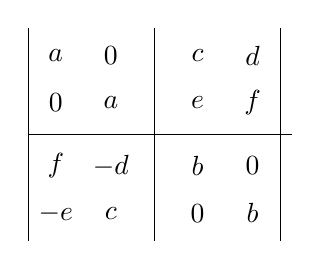
\begin{tikzpicture}
\node at (0,0) {$a$}; \node at (.7,0) {$0$}; \node at (1.8,0) {$c$}; \node at (2.5,0) {$d$};
\node at (0,-.6) {$0$}; \node at (.7,-.6) {$a$}; \node at (1.8,-.6) {$e$}; \node at (2.5,-.6) {$f$};
\node at (0,-1.4) {$f$}; \node at (.7,-1.4) {$-d$}; \node at (1.8,-1.4) {$b$}; \node at (2.5,-1.4) {$0$};
\node at (0,-2) {$-e$}; \node at (.7,-2) {$c$}; \node at (1.8,-2) {$0$}; \node at (2.5,-2) {$b$};
\draw (-.35,.35) -- (-.35,-2.35);
\draw (1.25,.35) -- (1.25,-2.35);
\draw (2.85,.35) -- (2.85,-2.35);
\draw (-.35,-1) -- (3,-1);
\end{tikzpicture}
\end{adjustbox}
\end{center}
Это условие на все $4\times4$ блоки

на диаг. скалярные;

симметричн. отн. диаг.
% Review region cancelled-word: bbox (1780,555,1970,620), inspected at 10x.
[Зачёркнуто: \Unclear{GELFAND-P000744}{cancelled-word}{неразборчивое слово}.]
связаны как выписано

\underline{Условия 1 и 2 опускаются} (они тоже могут быть выписаны).

Дальше: используются $e_{ij}$, но в ур-я они реально не входят.

\begin{equation*}
H\times S^4=L\oplus L^{\perp}
\end{equation*}
$L^{\perp}$ порождено глобально $2n$ сечениями расслоения $M\times S^4$;
% Review region bundle-letter: bbox (1790,1100,2085,1220), inspected at 10x.
\Unclear{GELFAND-P000744}{bundle-letter}{В этой строке записана буква $M$ в $M\times S^4$.}

\begin{align*}
(21)_1\qquad h_{k1}&=(x_2+ix_1)e_{k1}+(x_4-ix_3)e_{k2}+e_{k3}\\
(21)_2\qquad h_{k2}&=-(x_4+ix_3)e_{k1}+(x_2-ix_1)e_{k2}+e_{k4}
\end{align*}

% Column grouping review: bbox (220,1460,1010,2050), inspected at 3x.
\begin{equation*}
\underbrace{\begin{matrix}e_{k1}&e_{k2}\\\vphantom{\Large A}&\vphantom{\Large A}\end{matrix}}_{2n}
\quad\Bigg|\quad
\underbrace{\begin{matrix}e_{k3}&e_{k4}\\\vphantom{\Large A}&\vphantom{\Large A}\end{matrix}}_{2n}
\end{equation*}

На бесконечности всё тривиализуется.

«Инстантон живёт недолго и притом в мнимом времени —

— человекоподобное образование»

Выберем среди $e_{ij}$ базис $H$,\qquad $B\subset(e_{ij})$

$\Leftrightarrow$ $(2n+r)$-диагональный минор в $\widetilde Q$

(один такой минор)

По нему разложим систему порождающих сечений $L$.

\begin{equation*}
(22)\qquad\sum X_b\,Q\bigl(b,\underset{h_{k2}}{h_{k1}}\bigr)=0,\qquad k=1,\ldots,n;\qquad b\in B.
\end{equation*}
это система $2n$ ур-й для $2n+r$ неизвестных $X_b$.

Фунд. система решений $X^{(i)}$, $i=1,\ldots,r$.

Ортонормируем ее до $[Y^{(i)}]$ и теперь напишем ответ:

\SourcePage{GELFAND-P000745}{unlabelled}
% Original inspected directly, 2416 x 3472 pixels; coordinates use top-left origin.
% Text review at 3x: (110,45,2180,525), (235,510,1830,1220).
% Formula letters reviewed at 8x: (725,65,1210,210).
\begin{center}
\begin{adjustbox}{max width=\linewidth}
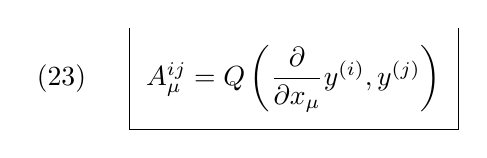
\begin{tikzpicture}
\node[inner sep=6pt] (a) {$A_{\mu}^{ij}=Q\left(\dfrac{\partial}{\partial x_{\mu}}y^{(i)},y^{(j)}\right)$};
\node[anchor=east] at ([xshift=-12pt]a.west) {$(23)$};
\draw (a.north west) -- (a.south west) -- (a.south east) -- (a.north east);
\end{tikzpicture}
\end{adjustbox}
\end{center}
\Unclear{GELFAND-P000745}{formula-y-case}{В формуле (23) обе буквы имеют строчную форму $y$.}

$X^{(i)}$ — рациональные ф-и со значениями в $H$;

при ортонормировании возникнут корни из рациональных ф-й.

\underline{Геометрическая теорема.}

Диаграммы $I\subset H\otimes\mathbb C^4$ с какими-то усл. \ldots

классифицируют расслоения над $\mathbb C P^3$ с условиями.

% First cohomology exponent inspected at 10x: bbox (490,835,700,935); visible dot and i stroke.
1) $H^i(L(-2))=0$ и то же для $L^*$;

2) $H^2(L(-1))=0$;

3) $H^0(L(-1))=0$.

\SourcePage{GELFAND-P000746}{15}
% Full original inspected at 2416 x 3472; review crop coordinates use original pixels.
% review heading bbox=(90,350,1750,680), 3x; handwritten label 15 bbox=(2230,30,2340,120).
\underline{28/$\overline{\underline{\mathrm{XI}}}$-77.}\qquad \underline{Сем. Гельфанда.}

% The speaker's name is doubly underlined and enclosed in a red rectangle in the source.
% review speaker-name bbox=(254,471,695,568), 3x.
\fbox{\underline{\underline{Л. Д. Фаддеев.}}}\qquad
\underline{Солитоны} \underline{как} \underline{частицы.}

I. $u(x,t)$ — поле, $x\in\mathbb{R}^{d}$, $d=1,2,3$.

% review equations-1-4 bbox=(90,660,1810,1700), 3x.
\begin{equation*}
\Box=\frac{\partial^{2}}{\partial t^{2}}-\frac{\partial^{2}}{\partial x^{2}}
\end{equation*}
\begin{equation*}
\Box u+m^{2}u+\varepsilon V'(u)=0
\tag{1}
\end{equation*}
\begin{equation*}
\mathcal{L}=\int\left[\frac{1}{2}\,\partial u\cdot\partial u
-\frac{1}{2}m^{2}u^{2}-\varepsilon V(u)\right]dx
\tag{2}
\end{equation*}
\begin{equation*}
\partial_{0}u(x,t)\underset{\mathrm{def}}{=}\pi(x,t)
\end{equation*}
\begin{equation*}
\{u(x,t),\pi(y,t)\}=\delta(x-y)
\tag{3}
\end{equation*}
% review hamiltonian-potential bbox=(1490,1500,1790,1680), 8x.
\begin{equation*}
H=\int\left[\frac{1}{2}\pi^{2}+\frac{1}{2}(\nabla u)^{2}
+\frac{1}{2}m^{2}u^{2}+\varepsilon V(u)\right]dx
\tag{4}
\end{equation*}

% Source has wavy underlining here and at the later textual subheadings.
% review free-field bbox=(105,1690,1970,2390), 3x.
\underline{Свободное поле}: $\varepsilon=0$

В квантовой теории $u,\pi$ — операторы.

Преобр. Фурье при $\varepsilon=0$:
\begin{equation*}
H=\int\sqrt{k^{2}+m^{2}}\,a^{*}(k)\,a(k)\,dk
\tag{5}
\end{equation*}
\begin{equation*}
\{a^{*}(k),a(k')\}=i\,\delta(k-k')
\tag{6}
\end{equation*}

% review quantization-and-spectrum bbox=(95,2360,2330,3280), 3x.
\underline{Квантование}: пусть $a,a^{*}$ — операторы, оператор
\begin{equation*}
\hat{\rho}(k)=\hat{a}^{*}(k')\hat{a}(k)
\tag{7}
\end{equation*}
% review eq7-argument bbox=(400,2490,1640,2630), 6x; GELFAND-0079-U400.
[\Unclear{GELFAND-P000746}{eq7-argument}{В первом множителе написано $\hat{a}^{*}(k')$.}]

имеет соб. значения:
\begin{equation*}
\rho'(k)=\sum\left[\delta(k-k_{1})+\dots+\delta(k-k_{n})\right]
\tag{8}
\end{equation*}
% review eq8-summation bbox=(335,2740,1550,2885), 6x and 8x; GELFAND-0079-U401.
[\Unclear{GELFAND-P000746}{eq8-summation}{Перед квадратной скобкой написан знак $\sum$ без пределов.}]

\underline{Спектр гамильтониана интерпретируется в терминах частиц.}
\begin{equation*}
E(k_{1},\dots,k_{n})=\omega(k_{1})+\dots+\omega(k_{n}),
\qquad \omega=\sqrt{k^{2}+m^{2}}
\tag{9}
\end{equation*}

(см.: аналогия с осциллятором)

\SourcePage{GELFAND-P000747}{unlabelled}
% Full original inspected at 2416 x 3472; no page label read in the frame.
% review top-text bbox=(210,15,2330,745), 3x; recheck bbox=(300,20,2170,365), 4x.
\underline{В классич. терминах}: если реш. с конечной энергией ур-я (1)
асимптотически приближ. на $\infty$ к реш. свободного ур-я, то эта
картина естественна.
% review top-cancelled-word bbox=(980,230,1145,300), 10x; GELFAND-0079-U402.
[Зачёркнуто: \Unclear{GELFAND-P000747}{top-cancelled-word}{Тогда?}]
Тогда $H(u)=H(u_{0})$, т. к. $H$ — интеграл.
% review integral-word bbox=(1700,225,2240,345), 8x.

Солитоны — контрпример к этой гипотезе.

\underline{Солитоны}: «всё, что не удовл. условию $u\to u_{0}$ при $|t|\to\infty$»

«Определение»: \underline{солитон — то, что}
% review definition-cancelled-start bbox=(355,560,620,657), 10x; GELFAND-0079-U403.
[Зачёркнуто: \Unclear{GELFAND-P000747}{definition-cancelled-start}{не уд}]
\underline{не расплывается на бесконечности, имея конечную энергию.}

% review example-and-lorentz-formula bbox=(140,735,2110,1380), 3x.
\underline{Пример}: решение стационарного ур-я.

$u_{s}(x)$ — одно решение $\Rightarrow$ преобр. Лоренца дает

% review eq10-deleted-factor bbox=(455,1110,590,1200), 10x; GELFAND-0079-U404.
[Перед левой скобкой зачёркнуто: \Unclear{GELFAND-P000747}{eq10-deleted-factor}{неразборчиво};
над зачёркнутым вписано $u_{s}$.]
\begin{equation*}
u_{s}\left(\frac{x-x_{0}-vt}{\sqrt{1-v^{2}}}\right)
=u_{s}(x,t\mid x_{0},v)
\tag{10}
\end{equation*}
% review eq10-right-correction bbox=(890,1000,1005,1245), 10x; GELFAND-0079-U405.
[\Unclear{GELFAND-P000747}{eq10-right-correction}{У правого конца дробной черты — небольшой зачёркнутый знак; правая скобка обведена и продлена вниз.}]

уже солитон, завис. от 2-х параметров.

% review asymptotics bbox=(145,1360,2090,2220), 3x.
При больших временах: если $v_{1}\ne v_{2}$ то
\begin{equation*}
u(x,t\mid x_{01},v_{1})+u(x,t\mid x_{02},v_{2})
\tag{11}
\end{equation*}
асимптотически решение.

Тогда асимптотика: при $|t|\to\infty$
\begin{equation*}
u\to u_{0}+\sum u(x,t\mid v_{i},x_{0i})
\tag{12}
\end{equation*}
% review eq12-argument-order bbox=(1170,1850,1480,1980), 3x and 10x; GELFAND-0079-U406.
[\Unclear{GELFAND-P000747}{eq12-argument-order}{После вертикальной черты написано $v_{i},x_{0i}$.}]

(в общем случае — гипотеза; в моделях — теорема)

При $t\to+\infty$ и при $t\to-\infty$ разные.

% review energy-and-quantization bbox=(150,2210,2280,3450), 3x.
Энергия
\begin{equation*}
H(u)=H(u_{0})+\sum_{i=1}^{n}H_{s}(v_{i})
\tag{13}
\end{equation*}
По релятив. ф-ле ясно, что
\begin{equation*}
H_{s}(v)=\frac{M}{\sqrt{1-v^{2}}}=\sqrt{p^{2}+M^{2}}
\qquad\text{(«энергия солитона»)}
\tag{14}
\end{equation*}

$M$ — энергия статич. солитона («масса» по определению).

(14) — определение $p$.

Получилось 2 части фазового пр-ва. Энергия:
\begin{equation*}
\int\omega(k)\rho(k)\,dk+\sum_{i}^{n}\sqrt{p_{i}^{2}+M^{2}}
\tag{15}
\end{equation*}

% review give-contribution bbox=(590,3150,1730,3260), 6x.
Солитоны дали вклад еще в классике. В квантовой
% review bottom-hbar bbox=(745,3260,2090,3420), 6x.
механике входит $\dfrac{M}{\hbar c}$; солитоны сохраняются при $\hbar\to+0$.
% GELFAND-0080. Дипломатическая транскрипция назначенных кадров.
% Оригинальные изображения просмотрены непосредственно; нерешённые чтения привязаны к журналу.
% Комментарии с координатами сохраняют воспроизводимость проверки после удаления временных вырезок.
\SourcePage{GELFAND-P000748}{16}
% Оригинал: chapter_012/12_part_000011.png; 2416 x 3472 пикселей.
% Координаты (x0,y0,x1,y1) в исходных пикселях от левого верхнего угла; правая и нижняя границы исключены.
% Масштаб — линейное увеличение вырезки при чтении; исходное разрешение не изменялось.
% Проверенная вырезка (200,40,2000,860), 3×.
% Проверенная вырезка (100,830,1900,1730), 3×.
% Проверенная вырезка (170,1710,2150,3070), 3×.
% Проверенная вырезка (870,560,978,690), 10×.
% Проверенная вырезка (410,865,1760,1090), 3×.
% Проверенная вырезка (45,690,1630,838), 3×.
% Проверенная вырезка (560,1510,1210,1730), 3×.
% Проверенная вырезка (480,1860,1230,1990), 4×.
% Проверенная вырезка (475,2500,785,2610), 6×.
% Проверенная вырезка (470,1230,600,1360), 8×.
% Проверенная вырезка (1270,900,1420,980), 10×.
% Проверенная вырезка (2110,3370,2416,3472), 5×.
% Проверенная вырезка (305,2845,725,2940), 4×.
% Проверенная вырезка (270,2850,1410,2985), 3×; повторная проверка names.
% Особенности исходного подчёркивания: Волнистые подчёркивания: «Периодич. решение.» и «Основная модельная задача:».
В квант. механике спектр. будет
\begin{equation*}
\sum_{i=1}^{N}\sqrt{k_i^2+m^2}+\sum_i^n\sqrt{p_i^2+M^2}
\tag{16}
\end{equation*}
Из одного поля 2 сорта частиц (по квазиклассике)

\underline{Периодич. решение.}
\begin{equation*}
u_p(x,t\mid x_0,\bar v,\Unclear{GELFAND-P000748}{eq17-beta}{\beta},\alpha)
\tag{17}
\end{equation*}
$\beta$ связано с $T$ (период), $\alpha$ (нач. фаза) параметры

В этом случае
\begin{equation*}
\sum_{i=1}^{N}\sqrt{\Unclear{GELFAND-P000748}{eq18-first-radicand}{k^2}+m^2}+\sum_i^n\sqrt{p_i^2+M^2}
+\sum_k^{\Unclear{GELFAND-P000748}{eq18-upper-index}{\tau\text{ или }r}}
\sqrt{p_k^2+\Unclear{GELFAND-P000748}{eq18-last-radicand}{M(\alpha_k)}}
\tag{18}
\end{equation*}

\underline{Основная модельная задача:}
\begin{equation*}
\Unclear{GELFAND-P000748}{eq19-potential-glyph}{v\text{ или }\upsilon}(u)=1-\cos u-\frac{u^2}{2}
\tag{19}
\end{equation*}
Ур-е имеет вид:
\begin{equation*}
\Box u+m^2\sin u=0
\tag{20}
\end{equation*}
(ур-е $(\sin\varphi)_2$)

Ещё один параметр: в скобке Пуассона поставим
\begin{equation*}
\{\partial_0u,u\}=\gamma\delta(\ldots)
\tag{21}
\end{equation*}
Тогда оказывается, что
\begin{equation*}
M=\frac{8m}{\gamma}\qquad\text{(„тяжёлая частица”)}
\tag{22}
\end{equation*}
\begin{equation*}
M_2(\alpha)=\frac{16m}{\gamma}\sin\alpha,\qquad 0<\alpha\leq\frac{\pi}{2}.
\tag{23}
\end{equation*}
Этими \Unclear{GELFAND-P000748}{cancelled-word}{[зачёркнуто: двумя?]} решениями всё определяется.

При этом надо брать
\begin{equation*}
\alpha=\frac{\gamma}{16}n,\quad n=1,2,\ldots
\tag{24}
\end{equation*}
(Тахтаджан, Фаддеев, $\approx 1974$ г.)

Сейчас должен выйти подробный обзор (по английски).

\SourcePage{GELFAND-P000749}{unlabelled}
% Оригинал: chapter_012/12_part_000012.png; 2416 x 3472 пикселей.
% Координаты (x0,y0,x1,y1) в исходных пикселях от левого верхнего угла; правая и нижняя границы исключены.
% Масштаб — линейное увеличение вырезки при чтении; исходное разрешение не изменялось.
% Проверенная вырезка (165,50,2180,405), 3×.
% Проверенная вырезка (345,380,1810,795), 3×.
% Проверенная вырезка (280,785,2175,1110), 3×.
% Проверенная вырезка (295,1110,1960,1680), 3×.
% Проверенная вырезка (290,1600,1915,2180), 3×.
% Проверенная вырезка (270,2090,2145,2800), 3×.
% Проверенная вырезка (150,2760,2160,3290), 3×.
% Проверенная вырезка (1090,180,1590,280), 5×.
% Проверенная вырезка (255,330,945,413), 4×.
% Проверенная вырезка (320,900,780,1100), 5×.
% Проверенная вырезка (800,888,1375,1020), 5×.
% Проверенная вырезка (860,800,1440,890), 5×.
% Проверенная вырезка (1190,1420,1610,1530), 5×.
% Проверенная вырезка (525,660,1350,800), 5×; повторная проверка eq26.
% Проверенная вырезка (230,170,2240,390), 3×; повторная проверка intro.
% Особенности исходного подчёркивания: Волнистые подчёркивания: заголовок раздела, Glimm, Jaffe, фамилия под ними, «Рассм. ур-е», «Тогда сущ. предел», отдельно «и» и «унитарный оператор». Короткое подчёркивание под II и подчёркивание у леммы 1 прямые.
\underline{II. Последовательное квантование и $S$-матрица.}

Найти настоящие сб. ф-и пока не удалось. Но $S$-матрица
вычислена! (обходным путем: континуальный интеграл)

Определения: написать
\begin{equation*}
H=\int\left[\frac{\pi^2}{2}+\frac{(\nabla u)^2}{2}+\frac{m^2}{2}u^2+V(u)\right]
\tag{25}
\end{equation*}
и считаем $\pi$ и $u$ операторами с соотношением
\begin{equation*}
[\hat\pi(x),\hat u(y)]=i\delta(x-y)
\tag{26}
\end{equation*}
Противоречия нет, но надо начать с перенормировок.

\underline{Glimm, Jaffe:}

\underline{\Unclear{GELFAND-P000749}{latin-surname}{Fröhlich / Frichlich}}
\begin{equation*}
\left[\begin{gathered}
\frac{m^2}{\gamma}(1-\cos\gamma u)\quad\text{при малых }\gamma\quad\text{построили}\\
\text{гамильтониан аккуратно}\quad\text{(при }x\in\mathbb{R}^1\text{).}
\end{gathered}\right.
\end{equation*}

\underline{Лемма 1} (из обычной квант. механики). \underline{Рассм. ур-е}
\begin{equation*}
i\frac{\partial\Psi}{\partial t}=H\Psi
\tag{27}
\end{equation*}
\begin{equation*}
H=-\frac{\Delta}{2m}+\Unclear{GELFAND-P000749}{eq28-potential}{v(x),\quad v\text{ (или }\upsilon\text{)}}\text{ быстро убывает}
\tag{28}
\end{equation*}
\underline{Тогда сущ. предел}
\begin{equation*}
S=\lim_{\substack{t''\to\infty\\t'\to-\infty}}
e^{iH_0t''}e^{-iH(t''-t')}e^{-iH_0t'}
\tag{29}
\end{equation*}
($S$-матрица) \underline{и} $S$ — \underline{унитарный оператор.}

Лучше считать в импульсном представлении: ядро
обозначается $S(p'',p')$. Достаточно знать ядро
опер. эволюции $e^{-iH(t''-t')}=K$
\begin{equation*}
K(x'',t''\mid x',t')
\end{equation*}
Надо взять
\begin{equation*}
\begin{cases}
x''=\dfrac{p''}{m}t''\\
x'=\dfrac{p'}{m}t'
\end{cases}
\tag{30}
\end{equation*}
(по классическим ф-лам со свободным $H_0$). Тогда
\begin{equation*}
S(p'',p')=\lim_{\substack{t''\to+\infty\\t'\to-\infty}}
\frac{K\left(\frac{p''}{m}t'',t''\mid\frac{p'}{m}t',t'\right)}
{K_0\left(\frac{p''}{m}t'',t''\mid0,0\right)K_0\left(0,0\mid\frac{p'}{m}t',t'\right)}
\tag{31}
\end{equation*}
(аналогична (29))

\SourcePage{GELFAND-P000750}{17}
% Оригинал: chapter_012/12_part_000013.png; 2416 x 3472 пикселей.
% Координаты (x0,y0,x1,y1) в исходных пикселях от левого верхнего угла; правая и нижняя границы исключены.
% Масштаб — линейное увеличение вырезки при чтении; исходное разрешение не изменялось.
% Проверенная вырезка (145,30,2330,410), 3×.
% Проверенная вырезка (60,395,2080,850), 3×.
% Проверенная вырезка (65,880,2260,1350), 3×.
% Проверенная вырезка (45,1330,2160,1940), 3×.
% Проверенная вырезка (260,1920,2170,2180), 3×.
% Проверенная вырезка (40,2190,2290,2700), 3×.
% Проверенная вырезка (155,2670,2295,3380), 3×.
% Проверенная вырезка (1800,390,2020,590), 8×.
% Проверенная вырезка (815,425,1010,555), 7×.
% Проверенная вырезка (435,1010,765,1140), 5×.
% Проверенная вырезка (1890,2240,2140,2390), 7×.
% Проверенная вырезка (250,2865,680,3020), 5×.
% Проверенная вырезка (170,3200,335,3340), 7×.
% Проверенная вырезка (505,2440,1120,2660), 4×.
% Проверенная вырезка (175,3200,2280,3435), 3×.
% Проверенная вырезка (1180,1420,1360,1520), 7×.
% Проверенная вырезка (1350,1430,1515,1545), 7×.
% Проверенная вырезка (548,2520,684,2640), 10×.
% Проверенная вырезка (410,710,1100,875), 4×; повторная проверка unnumbered-time-argument.
% Особенности исходного подчёркивания: Волнистые подчёркивания: «Комментарий к» и «Замолодчиков». Подчёркивание «Континуальный интеграл.» прямое.
Правая часть (31) считается континуальным интегралом по
траекториям с классическими асимптотиками.

\underline{Комментарий к} (31): применяем к $\Psi$, рассматривая волновой пакет
\begin{equation*}
\Psi(x,t)=\left[\frac{1}{2\pi}\int
\Unclear{GELFAND-P000750}{eq32-integrand-psi}{\Psi(p)\text{ (верхний штрих неясен)}}
e^{ipx}e^{-i\frac{p^2}{2m}t}\,dp\right]
\underset{\substack{\uparrow\\\text{метод стац.}\\\text{фазы}}}{\cong}
\tilde\Psi\left(\frac{mx}{t}\right)
e^{i\frac{x^2}{2m\Unclear{GELFAND-P000750}{eq32-exponent-overwrite}{t}}}
\tag{32}
\end{equation*}
\begin{equation*}
\Psi(t)=e^{-iH_0\Unclear{GELFAND-P000750}{unnumbered-time-argument}{t'}}\Psi
\end{equation*}
Получим
\begin{equation*}
K(.\ .\mid\frac{p}{m}t,t)\,\tilde\Psi(p)\sqrt{\frac{m}{t}}\,dp
\tag{33}
\end{equation*}
с множителями (в каждой части переходим в свою систему
координат). \tikz{\fill (0,0)--(0,0.22)--(0.25,0.11)--cycle;}

\underline{Континуальный интеграл.} Сначала для квантовой механики
\begin{equation*}
K(x'',t''\mid x',t')=\frac1N\int
 e^{i\int_{t'}^{t''}\left[\frac{m\dot x^2}{2}-\Unclear{GELFAND-P000750}{eq34-potential}{v\text{ или }\upsilon}(x)\right]dt}
 \prod_{t'\leq t\leq t''}dx(t),
\tag{34}
\end{equation*}
по таким траекториям, что
\begin{equation*}
x(t')=x',\quad x(t'')=x''
\tag{35}
\end{equation*}
$N$ — нормирующий множитель (зависящий от времени).

Теперь нужно считать, что $x(t')=\dfrac{pt'}m$, $x(t'')=\dfrac{pt''}m$.

В теории поля надо написать
\begin{equation*}
K(u''(x),t''\mid u'(x),t')=\frac1N\int\exp\left\{i\int\mathcal L(x)\,dx\right\}
\prod_{\substack{t'\leq t\leq t''\\-\infty<x<\infty}}
 du\,\Unclear{GELFAND-P000750}{eq36-cancelled-argument}{\text{[зачёркнуто: неразборчиво]}}(x,t)
\tag{36}
\end{equation*}
по таким $u$, что
\begin{equation*}
\begin{cases}
u(x,t'')=u''(x)\\
u(x,t')=u'(x)
\end{cases}
\tag{37}
\end{equation*}
В качестве нач. и конечных конфигураций надо взять
суммы по солитонам. Получаются вероятности перехода.

\Unclear{GELFAND-P000750}{good-word-crossing}{Хорошего [диагональный штрих поверх конца слова]}
квантового варианта обратной задачи пока нет.

Для $S$-матрицы $\sin$-Гордона угадана точная формула
(\underline{Замолодчиков} из ИТЭФ; см. Comm. on Math. Physics)

\Unclear{GELFAND-P000750}{hypothesis-prefixed-mark}{[зачёркнутый знак: неразборчиво]}
Гипотеза: все классич. решаемые задачи решаются и в квантовом
варианте

\SourcePage{GELFAND-P000751}{unlabelled}
% Оригинал: chapter_012/12_part_000014.png; 2416 x 3472 пикселей.
% Координаты (x0,y0,x1,y1) в исходных пикселях от левого верхнего угла; правая и нижняя границы исключены.
% Масштаб — линейное увеличение вырезки при чтении; исходное разрешение не изменялось.
% Проверенная вырезка (80,40,1150,220), 3×; top-formula.
% Проверенная вырезка (1080,180,2410,305), 3×; top-right.
% Проверенная вырезка (650,300,820,425), 5×; cancel-top.
% Проверенная вырезка (170,700,1630,820), 3×; eq39.
% Проверенная вырезка (320,815,840,915), 5×; cancel-operator.
% Проверенная вырезка (520,900,1410,1050), 5×; eq40.
% Проверенная вырезка (980,1250,2260,1380), 3×; later-loops.
% Проверенная вырезка (225,1720,640,1810), 5×; cancel-hope.
% Проверенная вырезка (300,1900,1330,2190), 3×; eq42-43.
% Проверенная вырезка (1210,2270,1600,2410), 5×; q-lower.
% Проверенная вырезка (850,2580,1040,2670), 8×; cancel-mass.
% Проверенная вырезка (500,2670,1410,3080), 3×; eq44-45.
% Проверенная вырезка (390,3110,2240,3335), 3×; bottom-line.
% Проверенная вырезка (300,490,1760,675), 3×; heading.
% Проверенная вырезка (1210,970,1285,1030), 10×; u-subscript.
% Проверенная вырезка (980,930,1080,1010), 10×; mass-operator-term.
% Проверенная вырезка (245,1615,730,1735), 3×; hope-title.
% Проверенная вырезка (690,1470,1260,1615), 4×; eq41.
% Проверенная вырезка (1240,3090,2070,3210), 3×; justified.
% Проверенная вырезка (340,2465,2160,2575), 3×; det-zero.
% Проверенная вырезка (790,1930,865,2010), 10×; q-comparison.
% Проверенная вырезка (320,815,840,915), 3×; дополнительное независимое чтение.
% Проверенная вырезка (320,825,580,900), 10×; дополнительное независимое чтение.
% Проверенная вырезка (550,825,840,900), 10×; дополнительное независимое чтение.
% Проверенная вырезка (455,835,710,900), 10×; дополнительное независимое чтение.
\begin{equation*}
\langle u''(x)\mid e^{-iH(t''-t')}\mid u'(x)\rangle
\tag{38}
\end{equation*}
— матр. элемент, задаваемый континуальным интегралом. Теперь надо делить и устремлять $t$ к $\pm\infty$.

Поправки к [зачёркнуто: \Unclear{GELFAND-P000751}{top-cancel}{неразборчиво}] классической массе возникают на уровне одного солитона.

\underline{Задачи, возникающие при вычислении интеграла.}

Метод стационарной фазы.
\begin{equation*}
u(x,t)=U_{cl}(x,t)+\sqrt h\,\varphi(x,t)+\ldots
\tag{39}
\end{equation*}
[Зачёркнуто: \Incomplete{GELFAND-P000751}{cancel-before-operator}{Текст перед словами «Возникает оператор» закрыт густым зачёркиванием и не разобран.}]
Возникает оператор
\begin{equation*}
A\varphi=\Box\varphi+m^2\Unclear{GELFAND-P000751}{operator-mass-term}{\varphi+}V''(\Unclear{GELFAND-P000751}{operator-u-index}{u_\varphi})\varphi
\tag{40}
\end{equation*}
Поправки вычисляются через $\det A$.

Он выражается через $S$-матрицу для вспомогательного линейного уравнения. Дальше петли возникают. Нужно знать обратный оператор $R=A^{-1}$ и ядро $\underline{R(x,y)}$, а именно
\begin{equation*}
\int R^3(x,x)\,d^2x
\tag{41}
\end{equation*}
\underline{Надежды:} не исключено, что такие функционалы явно считаются.

[Зачёркнуто: \Unclear{GELFAND-P000751}{cancel-quadratures}{в квадратурах}.]

Пусть $u_1$ — односолитонное решение (стационарное),
\begin{equation*}
V''(u_1(x))=q(x).
\tag{42}
\end{equation*}
Вычисление
\begin{equation*}
\det\left(\frac{d^2}{dt^2}-\frac{d^2}{dx^2}+q(x)\right)
\tag{43}
\end{equation*}
сводится к спектр. плотности стац. оператора (переменные разделяются). Получается $q(x)=\frac1{\operatorname{ch}^2 x}$ и явно находятся все соб. функции (простейший потенциал Баргмана).

$\det A$ выраж. через соб. ф-ю с нулевым соб. значением.

Поправки к массе [зачёркнуто: \Unclear{GELFAND-P000751}{cancel-before-soliton}{неразборчиво}] солитона:
\begin{equation*}
M=\frac{8m}{\gamma}-\frac m\pi+O(\gamma)
\tag{44}
\end{equation*}
\underline{Гипотеза:} для sine-Gordon
\begin{equation*}
M=\frac{8m}{\gamma}-\frac m\pi,
\tag{45}
\end{equation*}
т.е. высших поправок нет. (\Unclear{GELFAND-P000751}{justified-abbreviation}{оправд.} Замолодчиковым)

При $\gamma\le8\pi$ всё хорошо, а дальше солитон исчезает.

\SourcePage{GELFAND-P000752}{18}
% Оригинал: chapter_012/12_part_000015.png; 2416 x 3472 пикселей.
% Координаты (x0,y0,x1,y1) в исходных пикселях от левого верхнего угла; правая и нижняя границы исключены.
% Масштаб — линейное увеличение вырезки при чтении; исходное разрешение не изменялось.
% Проверенная вырезка (2310,0,2416,110), 5×; label.
% Проверенная вырезка (375,275,875,430), 5×; eq46-left.
% Проверенная вырезка (865,275,1840,430), 3×; eq46-right.
% Проверенная вырезка (360,600,1310,850), 4×; eq47.
% Проверенная вырезка (215,860,1270,990), 5×; cancel-47.
% Проверенная вырезка (380,1150,1325,1310), 4×; eq48.
% Проверенная вырезка (225,1310,2340,1415), 3×; zamolod.
% Проверенная вырезка (470,1630,1160,1830), 5×; eq49.
% Проверенная вырезка (220,1830,1270,1950), 4×; cancel-eigen.
% Проверенная вырезка (390,2280,1100,2430), 4×; eq51.
% Проверенная вырезка (270,2490,2170,2715), 3×; names.
% Проверенная вырезка (1430,0,1540,125), 6×; visible-label.
% Проверенная вырезка (640,290,700,430), 10×; separator46.
% Проверенная вырезка (680,1820,1260,1955), 6×; canceled-eigen-right.
% Проверенная вырезка (995,2490,1335,2645), 6×; pohlmeyer-prefix.
% Проверенная вырезка (270,2610,640,2725), 6×; canceled-quantum.
% Проверенная вырезка (250,1940,1300,2130), 3×; lower-heading.
% Проверенная вырезка (445,1535,510,1600), 10×; cancel-system.
% Проверенная вырезка (2220,20,2335,120), 6×; label-final.
% Проверенная вырезка (230,860,735,1010), 6×; cancel47-left.
% Проверенная вырезка (710,860,1280,1010), 6×; cancel47-right.
% Проверенная вырезка (230,1830,815,1955), 6×; cancel49-prefix.
% Проверенная вырезка (1820,1430,2330,1530), 3×; quantum-abbrev.
% Проверенная вырезка (275,2410,1820,2520), 3×; nontrivial.
% Проверенная вырезка (0,0,2416,200), 1×; top-strip.
% Проверенная вырезка (940,1640,1040,1750), 10×; potential-numerator.
% Проверенная вырезка (940,1640,1040,1750), 10×; повторная проверка eq49-numerator.
% Проверенная вырезка (215,860,1280,1010), 3×; дополнительное независимое чтение.
% Проверенная вырезка (850,870,1280,990), 10×; дополнительное независимое чтение.
% Проверенная вырезка (1050,875,1245,995), 10×; дополнительное независимое чтение.
% Проверенная вырезка (220,1830,1270,1955), 3×; дополнительное независимое чтение.
% Проверенная вырезка (865,1830,1270,1955), 10×; дополнительное независимое чтение.
% Проверенная вырезка (1010,1840,1240,1940), 10×; дополнительное независимое чтение.
\underline{Формулы $S$-матрицы для sin-Гордона.}

Надо Сосчитать укороченное действие для 2-солитонного решения.
\begin{equation*}
S_{sa}(p_1'',p_2''\Unclear{GELFAND-P000752}{equation-46-separator}{;}p_1',p_2')=
\delta(p_1''-p_1')\delta(p_2''-p_2')e^{i\Theta(p_1,p_2)}
\tag{46}
\end{equation*}
(Есть солитон и антисолитон)

Действие (классическое)
\begin{equation*}
\Theta=\frac8\gamma\int_0^\pi d\alpha\left[\ln\frac{e^{i(\beta-\alpha)}+1}{e^{i\beta}+e^{-i\alpha}}\right]
\tag{47}
\end{equation*}
[Зачёркнуто: При $\gamma=\frac{8\pi}{N}$, $N$ — целое \Incomplete{GELFAND-P000752}{cancel-after-47}{Конец зачёркнутой строки после «целое» неразборчив.}]
(интеграл не берётся).

Надо взять $\gamma=\frac{8\pi}{N}$, $N$ — целое число
\begin{equation*}
\Theta\longrightarrow\sum\ln(\ldots)
\tag{48}
\end{equation*}
Замолодчиков считал, что это верно для $\gamma=\frac{8\pi}{N}$ и проинтерполировал.

В результате sin-Гордон оказался похож на квантовомеханич. систему [зачёркнуто: и] с
\begin{equation*}
H=-\frac{d^2}{dx^2}+\frac{\Unclear{GELFAND-P000752}{potential-numerator}{a}}{\operatorname{ch}^2\alpha x}
\tag{49}
\end{equation*}
[Зачёркнуто: Соб. значение $\Unclear{GELFAND-P000752}{cancel-eigenvalue-formula}{\alpha(\ell+\frac12)^2}$ \Incomplete{GELFAND-P000752}{cancel-eigenvalue-end}{Конец зачёркнутой строки не разобран; виден фрагмент «с пр…».}]

\underline{Замечательная дин. система}

связана с полем (киральным)
\begin{equation*}
n(x):R^2\longrightarrow S^n\subset R^{n+1}
\tag{50}
\end{equation*}
\begin{equation*}
\mathcal L=\frac12\int\partial n\cdot\partial n\,dx
\tag{51}
\end{equation*}
нетривиален из-за значений (есть нелинейность).

$L$-$A$ пара написана ([зачёркнуто: \Unclear{GELFAND-P000752}{name-correction}{Фоль}; надписано: Поль]майер (?); Захаров и Михайлов)

[Зачёркнуто: На \Incomplete{GELFAND-P000752}{cancel-before-quantization}{Продолжение после «На» перед словом «Квантование» закрыто густым зачёркиванием и не разобрано.}]
Квантование слабо связано с классикой.

Массивные частицы появляются как солитоны.

По этому поводу будет доклад на сем. им. И.Г. Петровского.

\SourcePage{GELFAND-P000753}{unlabelled}
% Оригинал: chapter_012/12_part_000016.png; 2416 x 3472 пикселей.
% Координаты (x0,y0,x1,y1) в исходных пикселях от левого верхнего угла; правая и нижняя границы исключены.
% Масштаб — линейное увеличение вырезки при чтении; исходное разрешение не изменялось.
% Проверенная вырезка (185,55,1080,180), 3×; heading.
% Проверенная вырезка (200,190,2330,280), 3×; first-comment.
% Проверенная вырезка (240,345,1980,440), 3×; problem-line.
% Проверенная вырезка (295,795,2290,895), 3×; grassmann-line.
% Проверенная вырезка (270,890,1480,1110), 4×; exterior-relations.
% Проверенная вырезка (1480,1200,2130,1290), 5×; grading-cancel.
% Проверенная вырезка (270,1310,1780,1455), 3×; grading-basis.
% Проверенная вырезка (285,1450,2020,1620), 3×; object-text.
% Проверенная вырезка (270,2110,2320,2290), 3×; complex-text.
% Проверенная вырезка (120,3035,1910,3380), 3×; homology-bottom.
% Проверенная вырезка (1815,345,1885,425), 10×; cancel-pn.
% Проверенная вырезка (385,495,470,595), 8×; affine-symbol.
% Проверенная вырезка (365,445,1910,780), 3×; projective-definition.
% Проверенная вырезка (1880,795,1955,860), 10×; cancel-algebra.
% Проверенная вырезка (440,1350,535,1445), 10×; cancel-lambda-k.
% Проверенная вырезка (175,1650,2010,2120), 3×; eq2-4.
% Проверенная вырезка (295,2835,1515,3040), 3×; definition-proper.
% Проверенная вырезка (115,3080,210,3180), 10×; number7.
% Проверенная вырезка (350,3080,440,3185), 10×; cancel-hi.
% Проверенная вырезка (355,3190,1015,3325), 5×; cancel-homology.
% Проверенная вырезка (565,606,625,675), 10×; scalar-left.
% Проверенная вырезка (745,608,805,675), 10×; scalar-right.
% Проверенная вырезка (345,3195,1045,3310), 8×; homology-final.
\underline{13/II - 78 г.}\qquad\underline{Сем. Гельфанда.}

\underline{И.М.Г.} В теории категорий есть 2 перв. понятия: 1) Topos 2) Производная категория

\begin{adjustbox}{max width=\linewidth}
\begin{tikzpicture}[baseline]
\node[draw=red,rectangle,inner sep=3pt,anchor=base] {\underline{С. Гельфанд}};
\end{tikzpicture}
\end{adjustbox}.

\underline{Задача:} описать все алгебраические расслоения над [зачёркнуто: \Unclear{GELFAND-P000753}{cancel-before-projective}{неразборчивый знак}] $\mathbb P^n$.

($n$-мерное проект. пр-во; например, над $\mathbb C$).

$\Xi$ — аффинное пр-во
\begin{equation*}
\xi\sim\alpha\xi,\quad\alpha\in\mathbb C^*;\qquad\text{тогда }\Xi/{\sim}=\mathbb P^n
\end{equation*}
$(\xi\ne0)$

$\Lambda$ — грассманова алгебра от $(n+1)$-го переменного ([зачёркнуто: \Unclear{GELFAND-P000753}{cancel-before-algebra}{неразборчиво}] алг. над $\Xi$).
\begin{equation*}
\Lambda=\{\xi_0,\ldots,\xi_n\mid\xi_i\xi_j+\xi_j\xi_i=0\}.
\end{equation*}
\begin{equation*}
\dim\Lambda=2^{n+1}.
\end{equation*}
Введём на $\Lambda$ градуировку
\begin{equation*}
\Lambda=\Lambda_0\oplus\Lambda_{-1}\oplus\ldots\oplus\Lambda_{-(n+1)},
\tag{1}
\end{equation*}
[Справа зачёркнуто: $\Lambda_0$ — поле констант]

где
\begin{equation*}
\Lambda_{-k}\quad
\text{[зачёркнуто: }\Unclear{GELFAND-P000753}{cancel-grading-symbol}{\Lambda_k}\text{]}
=\{\xi_{i_1}\ldots\xi_{i_k}\},\quad\Lambda_0\text{ — поле констант}.
\end{equation*}
\underline{Объект:} градуир. конечномерное представление $\Lambda$ или градуир. $\Lambda$-модуль:
\begin{equation*}
V=\bigoplus V_j,\qquad\dim V<\infty.
\tag{2}
\end{equation*}
\begin{equation*}
\Lambda_{-k}V_j\subset V_{j-k}
\tag{3}
\end{equation*}
Пусть $\xi_0,\ldots,\xi_n$ — базис в $\Xi$, $\xi\in\Xi$.
\begin{equation*}
\xi=c_0\xi_0+\ldots+c_n\xi_n
\tag{4}
\end{equation*}
$(-k)$ — по историческим причинам (от статьи Серра)

Тогда $\xi:V_j\longrightarrow V_{j-1}$. Отсюда т.к. $\operatorname{deg}\xi=-1$, то
\begin{center}
\begin{adjustbox}{max width=\linewidth}
\begin{tikzcd}[column sep=large]
\ldots\arrow[r]&V_1\arrow[r,"\xi"]&V_0\arrow[r,"\xi"]&V_{-1}\arrow[r]&\ldots
\end{tikzcd}
\end{adjustbox}
\end{center}
$\xi^2=0\quad\Rightarrow\quad$ получили комплекс

Итак,

По элементу $\xi\ne0$ и модулю $V$ строится комплекс
\begin{equation*}
L_\xi(V)=\{\ldots\longrightarrow V_1\overset{\xi}{\longrightarrow}V_0\overset{\xi}{\longrightarrow}V_{-1}\longrightarrow\ldots\}
\tag{5}
\end{equation*}
\underline{Определение.} $V$ наз. \underline{правильным}, если
\begin{equation*}
\forall\xi\ne0,\qquad H_i(L_\xi(V))=0\quad\text{при }i\ne0
\tag{6}
\end{equation*}
Здесь:
\begin{equation*}
H_i\quad\text{[зачёркнуто: }\Unclear{GELFAND-P000753}{cancel-homology-symbol}{\text{неразборчивый знак}}\text{]}
(L_\xi(V))=\ker(V_i\to V_{i-1})/\operatorname{Im}(V_{i+1}\to V_i)
\tag{\Unclear{GELFAND-P000753}{homology-equation-number}{7}}
\end{equation*}
— [зачёркнуто: \Unclear{GELFAND-P000753}{cancel-homology-word}{факторпространства}] \underline{гомологии комплекса}

\SourcePage{GELFAND-P000754}{43}
% Оригинал: chapter_012/12_part_000017.png; 2416 x 3472 пикселей.
% Координаты (x0,y0,x1,y1) в исходных пикселях от левого верхнего угла; правая и нижняя границы исключены.
% Масштаб — линейное увеличение вырезки при чтении; исходное разрешение не изменялось.
% Проверенная вырезка (160,0,1620,690), 3×.
% Проверенная вырезка (210,650,700,800), 5×.
% Проверенная вырезка (135,740,2270,1530), 3×.
% Проверенная вырезка (180,1490,1350,1900), 3×.
% Проверенная вырезка (1250,1490,2210,1900), 3×.
% Проверенная вырезка (170,1900,1860,2240), 3×.
% Проверенная вырезка (160,2200,2300,2520), 3×.
% Проверенная вырезка (65,2500,1420,2920), 3×.
% Проверенная вырезка (1300,2510,2330,2770), 3×.
% Проверенная вырезка (55,2880,1880,3410), 3×.
% Проверенная вырезка (620,110,720,190), 10×.
% Проверенная вырезка (1390,395,1510,490), 10×.
% Проверенная вырезка (770,1960,950,2050), 7×.
% Проверенная вырезка (265,380,1540,575), 3×.
В этом случае
\begin{equation*}
\dim \Unclear{GELFAND-P000754}{top-homology-mark}{H_0^{\bullet}}(L_\xi(V))=\mathrm{const}
\end{equation*}
(не зависит от $\xi$)

в силу формулы Эйлера

(лев. часть — эйлерова характеристика\Unclear{GELFAND-P000754}{euler-overwritten-mark}{[переписанный знак, возможно $\xi$]}.
равная $\sum(-1)^i\dim V_i$.)

Расслоение: $\xi\mapsto H_0(L_\xi(V))$

\Unclear{GELFAND-P000754}{cancelled-line}{[Зачёркнуто: «Если $\xi$ и»; чтение неуверенно.]}

Для $\xi$ и $\alpha\xi$ одно и то же (есть естеств. изоморфизм).

\underline{Пример.} $V=\Lambda$ (регулярное представление).

$V_j=\Lambda_j$ (градуировка та же, что была).

\underline{Ответ:} $H_i(L_\xi(V))=0$, $\forall i$, $\forall\xi\ne0$.

Получаем нулевое расслоение.

Прямые суммы дадут тот же результат.

$V_j=\Lambda_{j+\ell}$ ($\ell$ — фиксировано)

$\Rightarrow$ снова получаем трив. расслоение.

Отсюда свб. модули приводят к трив. расслоениям.

% The theorem heading has a double underline; its statement has a wavy underline.
\underline{Теорема 1} Любое расслоение получ. такой конструкцией,
причём $V$ определено однозначно с точностью до добавления
свободного модуля.

(Бернштейн, С. Гельфанд, И. Гельфанд;
независимо близкий рез. Бейлинсон, студ. 3-го курса)

\underline{Уточнение конструкции расслоения.}

$V$ — произвольный $\Lambda$-модуль.

$O(k)$ — стандартные расслоения (их сеч. — однородные рац. ф-и
степени $k\in\mathbb{Z}$), одномерные.

Рассмотрим
\begin{equation*}
\mathcal{L}_j=V_{-j}\otimes O(j).\tag{8}
\end{equation*}
— расслоение над $\mathbb{P}^n$; каждый слой умножается на $V_{-j}$.

$O(1)$ — то, у которого есть сечение.

Построим
\begin{equation*}
d:\mathcal{L}_j\longrightarrow\mathcal{L}_{j+1}.\tag{9}
\end{equation*}
$f(\xi)$ — сеч. $\mathcal{L}_j$ над открытым мн-вом

однор. ф-я степ. $j$ со знач. в $V_{-j}$
\begin{equation*}
d(f(\xi))=\xi(f(\xi)).\tag{10}
\end{equation*}
(справа действие $\xi$ на $V_{-j}$, дающее $V_{-j-1}$).

\SourcePage{GELFAND-P000755}{unlabelled}
% Оригинал: chapter_012/12_part_000018.png; 2416 x 3472 пикселей.
% Координаты (x0,y0,x1,y1) в исходных пикселях от левого верхнего угла; правая и нижняя границы исключены.
% Масштаб — линейное увеличение вырезки при чтении; исходное разрешение не изменялось.
% Проверенная вырезка (2110,0,2416,180), 3×.
% Проверенная вырезка (45,25,2330,365), 3×.
% Проверенная вырезка (210,305,2280,745), 3×.
% Проверенная вырезка (210,725,2370,1220), 3×.
% Проверенная вырезка (95,1185,1890,1610), 3×.
% Проверенная вырезка (80,1610,2180,2250), 3×.
% Проверенная вырезка (170,2260,2210,2720), 3×.
% Проверенная вырезка (110,2680,2360,3090), 3×.
% Проверенная вырезка (100,3080,1670,3440), 3×.
% Проверенная вырезка (1495,160,1655,300), 8×.
% Проверенная вырезка (1495,160,1655,300), 10×.
% Проверенная вырезка (370,1060,520,1170), 8×.
% Проверенная вырезка (1390,2120,1790,2270), 6×.
% Проверенная вырезка (370,2030,630,2160), 6×.
% Проверенная вырезка (525,2060,635,2150), 10×.
% Проверенная вырезка (1850,2890,2370,3120), 5×.
% Проверенная вырезка (1910,2910,1990,3010), 10×.
% Проверенная вырезка (190,160,710,305), 5×.
% Проверенная вырезка (225,200,475,285), 10×.
% Проверенная вырезка (190,160,710,305), 5×; повторная проверка complex-start.
$O(1)$ — расслоение Хопфа. (или $O(-1)$). Получаем комплекс
\begin{equation*}
\{\ldots\longrightarrow\mathcal{L}_{-1}\overset{d}{\longrightarrow}\mathcal{L}_0
\overset{d}{\longrightarrow}\mathcal{L}_1\longrightarrow\ldots\}
=\mathcal{L}(V)\Unclear{GELFAND-P000755}{complex-end-mark}{\xi}.\tag{11}
\end{equation*}
над каждой точкой $\xi$ будет тот же самый комплекс, что и
раньше (легко проверить)

\underline{Утверждение:} если $V$ — правильное, то $H^0(\mathcal{L}(V))$ — расслоение и
$H^i(\mathcal{L}(V))=0$ при $i\ne0$.

Положим
\begin{equation*}
\Phi(V)=H^0(\mathcal{L}(V)).\tag{12}
\end{equation*}
% The heading and statements are underlined in the source.
\underline{Теорема $1'$.} 1) Каждое рассл. есть $\Phi(V)$ для некоторого правильного $V$

2) $\Unclear{GELFAND-P000755}{functor-letter-variation}{\varphi(V)}\approx\Phi(V')\Leftrightarrow\exists$ свободные $P$, $P'$:
$V\oplus P\cong V'\oplus P'$.

\underline{Обратное отображение.}

По расслоению надо построить $\Lambda$-модуль $V$.
\begin{equation*}
\underset{\text{рассл.}}{\mathcal{E}}\rightsquigarrow\mathcal{E}\otimes O(1)\tag{13}
\end{equation*}
чему это соотв. в $\Lambda$-модулях?

Пусть есть точная послед. $\Lambda$-модулей
\begin{equation*}
0\longrightarrow\underset{\text{прав.}}{V}\longrightarrow
\underset{\text{своб.}}{P}\longrightarrow V'\longrightarrow0\tag{14}
\end{equation*}
Постр. $W$ \Unclear{GELFAND-P000755}{w-construction-mark}{[малый знак, возможно $\circ$]};
$W_j=V'_{j+1}$.

\begin{equation*}
\text{Утв.:}\quad W\text{ — правильный и }\varphi(W)=\varphi(V)\otimes O(1)\tag{15}
\end{equation*}
Пусть $\mathcal{E}$ — расслоение; рассмотрим $\mathcal{E}\otimes O(N)$ при
достаточно большом $N$. Теорема Серра: расслоение
$\mathcal{E}\otimes O(N)$ имеет много сечений („обильное расслоение“),
они проводятся через любую точку в любом слое.

Рассм. $C_N=\Gamma(\mathbb{P}^n,\mathcal{E}\otimes O(N))$;
\begin{equation*}
\dim\Gamma(\mathbb{P}^n,O(1))=n+1\tag{16}
\end{equation*}
(линейные ф-и от $\xi$)

$\xi_0,\ldots,\xi_n$ — базис в $\Xi$

$x_0,\ldots,x_n$ — дуальный базис в $\Gamma(\mathbb{P}^n,O(1))$
(\Unclear{GELFAND-P000755}{linear-space-cancelled-mark}{[зачёркнутый знак, возможно «в»]} это пр-во линейных ф-ий)

(коэфф. разложения по предыд. базису)

Имеются операторы
\begin{equation*}
X_i:C_N\longrightarrow C_{N+1},\quad i=0,1,\ldots,n.\tag{17}
\end{equation*}
(умножение на $x_i$)

\SourcePage{GELFAND-P000756}{44}
% Оригинал: chapter_012/12_part_000019.png; 2416 x 3472 пикселей.
% Координаты (x0,y0,x1,y1) в исходных пикселях от левого верхнего угла; правая и нижняя границы исключены.
% Масштаб — линейное увеличение вырезки при чтении; исходное разрешение не изменялось.
% Проверенная вырезка (95,35,2140,475), 3×.
% Проверенная вырезка (75,435,1630,740), 3×.
% Проверенная вырезка (210,730,2350,1210), 3×.
% Проверенная вырезка (130,1190,2350,1560), 3×.
% Проверенная вырезка (240,1550,2380,1885), 3×.
% Проверенная вырезка (220,1850,2000,2290), 3×.
% Проверенная вырезка (160,2280,2310,2610), 3×.
% Проверенная вырезка (1140,270,1240,365), 10×.
% Проверенная вырезка (1380,1395,1545,1490), 10×.
% Проверенная вырезка (1480,1530,2370,1850), 4×.
% Проверенная вырезка (270,1730,355,1840), 10×.
% Проверенная вырезка (1500,1810,1615,1885), 10×.
% Проверенная вырезка (365,2100,635,2220), 7×.
% Проверенная вырезка (365,2100,635,2220), 10×.
% Проверенная вырезка (680,2100,1840,2350), 3×.
% Проверенная вырезка (1070,1970,1660,2100), 5×.
Построим теперь 2 $\Lambda$-модуля
\begin{equation*}
V=C_N\otimes\Lambda\tag{18}
\end{equation*}
(на $C_N$ трив. действие \Unclear{GELFAND-P000756}{action-overwritten-symbol}{$\Xi$}; на $\Lambda$ обычное действие)
\begin{equation*}
V'=C_{N+1}\otimes\Lambda.\tag{18'}
\end{equation*}
Имеем
\begin{equation*}
\partial:V\longrightarrow V'\tag{19}
\end{equation*}
\begin{equation*}
\partial(c\otimes\lambda)=\sum_{i=0}^{n}X_i(c)\otimes\xi_i\lambda\tag{20}
\end{equation*}
От базиса $\partial$ не зависит. Положим $W=\operatorname{Ker}\partial$.

Это $\Lambda$-модуль. Теперь надо сдвинуться обратно $N$ раз
\begin{equation*}
0\longrightarrow W'\longrightarrow P\longrightarrow W\longrightarrow0
\end{equation*}
$W\mapsto W'$ проделать $N$ раз (со сдвигом градуировки).

Это и есть то самое представление (тот самый $\Lambda$-модуль)

\underline{И.М.Г.} \underline{Классиф. расслоений} — не совсем прав. задача (не образуют абелеву
категорию). Надо разрешить слоям менять \Unclear{GELFAND-P000756}{cancelled-dimension-word}{[зачёркнутое слово неразборчиво]}
размерность — ввести пучки. Излаг. работа — развитие теор. Серра.

\underline{Теорема Серра}
% The parenthesized word (градуир.) is inserted above модули.
% The source has an oblique slash before the four-line right-hand qualification.
\begin{equation*}
\{\text{Пучки на }\mathbb{C}P^n\}\Leftrightarrow
\left\{
\begin{array}{l}
\text{конечно-порожд. }\overset{\text{(градуир.)}}{\text{модули}}\\
\text{над }\mathbb{C}[x_0,\ldots,x_n]
\end{array}
\Big/
\begin{array}{l}
\text{с точн.}\\
\text{до конечн.}\\
\text{числа однор.}\\
\text{компонент}
\end{array}
\right\}
\end{equation*}
\Unclear{GELFAND-P000756}{book-left-mark}{[переписанный знак, возможно $\xi$]}
(статья в сб. „Расслоенные пр-ва“; 1953 года).
\Unclear{GELFAND-P000756}{book-right-cancellation}{[зачёркнутый фрагмент неразборчив]}

Построим пучок по модулю $M$.

Зададим его сечения над $E_i=\{x.\ x_i\ne0\}$

\Unclear{GELFAND-P000756}{cancelled-section-formula}{[зачёркнутая формула, возможно $\Gamma(E_i,M)$]}
\begin{equation*}
\Gamma(E_i,\underset{\text{наш пучок}}{L})
=\left\{\frac{m}{x_i^s},\ \begin{array}{l}\operatorname{deg}m=s\\m\in M\end{array}\right\}.
\end{equation*}
$O(N)$ возникает из $M=\mathbb{C}[x_0,\ldots,x_n]$ со сдвинутой
градуировкой
\begin{equation*}
M_i=\{\mathbb{C}[x_0,\ldots,x_n]\}_{i+N}.
\end{equation*}

\SourcePage{GELFAND-P000757}{unlabelled}
% Оригинал: chapter_012/12_part_000020.png; 2417 x 3473 пикселей.
% Координаты (x0,y0,x1,y1) в исходных пикселях от левого верхнего угла; правая и нижняя границы исключены.
% Масштаб — линейное увеличение вырезки при чтении; исходное разрешение не изменялось.
% Прямо просмотрен весь оригинал 2417 x 3473; верхняя часть до y=2110 свободна от рукописного текста.
% Координаты проверенных областей: (150,2110,1240,2380) 3x; (200,2345,1470,2525) 3x;
% (1420,2345,2370,2470) 3x; (190,2530,740,2835) 4x; (180,2740,565,2825) 8x;
% (195,2750,310,2815) 10x; (520,2740,1220,2885) 3x; (220,2880,1420,3180) 3x;
% (215,3155,1190,3435) 3x; (1150,3155,2400,3310) 3x. Начало координат — левый верхний угол.

\underline{\underline{27/II-78}} г. \qquad \underline{Сем. Гельфанда.}

С. И. Гельфанд.
[Имя подчёркнуто волнистой линией и заключено в красную прямоугольную рамку.]

Задача: описать алгебраические векторные расслоения над проективным
пр-вом. [Слово «Задача» подчёркнуто волнистой линией.]

$\Xi$ — $(n+1)$-мерное пространство (векторное).

$\mathbb{P}=\mathbb{P}(\Xi)$ — проективное $n$-мерное пространство

[Зачёркнуто: \Unclear{GELFAND-P000757}{cancelled-word}{неразборчивое слово}.]
Выберем базис $\Xi$: $\xi_0,\ldots,\xi_n$
и пусть
\begin{equation*}
\Lambda=\Lambda(\Xi)\quad\text{— внешняя алгебра }\Xi
\end{equation*}
\begin{equation*}
\Lambda=\bigoplus_{i=-n-1}^{0}\Lambda_i
\end{equation*}
$\Lambda$ имеет образующие $\xi_0,\ldots,\xi_n$ и соотношения
$\xi_i\xi_j+\xi_j\xi_i=0$, $\xi_i^2=0$,
\begin{equation*}
\Lambda_{-k}=\{\xi_{i_1}\ldots\xi_{i_k}\}
\end{equation*}
% GELFAND-0081. Дипломатическая транскрипция десяти исходных кадров.
% Редакторские описания помещены в квадратные скобки или в общие маркеры неопределённости.
% Координаты просмотров даны в пикселях оригинала [left,top,right,bottom);
% xN — кратность увеличения, без добавления новых исходных пикселей.
\SourcePage{GELFAND-P000758}{unlabelled}
% Повторные просмотры исходного кадра:
% основной просмотр; 758-note-top: [250,185,2330,365) x3.
% основной просмотр; 758-definitions: [230,980,2020,1535) x3.
% основной просмотр; 758-l-correction: [270,1620,1910,2110) x3.
% основной просмотр; 758-cancellation: [235,2990,1870,3230) x3.
% основной просмотр; 758-cancel-symbols: [640,3065,1020,3185) x7.
% основной просмотр; 758-bottom: [105,3200,1740,3400) x3.
% основной просмотр; 758-cancellation-right: [1120,3050,1850,3200) x5.
% основной просмотр; 758-index-correction: [560,1690,710,1840) x8.
% основной просмотр; 758-section-formulas: [300,2280,1730,2660) x3.
% основной просмотр; 758-sections-index: [560,1950,790,2105) x8.
% основной просмотр; 758-parenthetical-i: [1230,297,1330,355) x8.
% основной просмотр; 758-cancelled-p: [835,3050,1210,3180) x6.
% независимая проверка; 758-topremark: [1190,265,2265,372) x3.
% независимая проверка; 758-sections: [410,1915,1900,2112) x3.
% независимая проверка; 758-v-index: [1560,1915,1760,2040) x10.
% независимая проверка; 758-tensor: [285,1620,1895,1840) x3.
% независимая проверка; 758-bottomcancel: [745,3080,1810,3190) x6.
% независимая проверка; 758-sootn: [1960,267,2225,354) x8.
% независимая проверка; 758-transitions: [1180,965,1590,1100) x6.
% независимая проверка; 758-cancel-left: [850,3085,1135,3170) x10.
% независимая проверка; 758-cancel-right: [1080,3080,1775,3200) x8.
% независимая проверка; 758-cancel-tops: [850,3020,1260,3200) x6.
% Координаты областей: пиксели исходного PNG, начало в левом верхнем углу;
% прямоугольники [x0,y0,x1,y1). Просмотрен весь оригинал 2416 x 3472.
% Повторные просмотры: [250,185,2330,365) x3;
% [230,980,2020,1535) x3; [270,1620,1910,2110) x3;
% [560,1690,710,1840) x8; [560,1950,790,2105) x8;
% [300,2280,1730,2660) x3;
% [235,2990,1870,3230) x3; [640,3065,1020,3185) x7;
% [1120,3050,1850,3200) x5; [105,3200,1740,3400) x3;
% [1230,297,1330,355) x8; [835,3050,1210,3180) x6.
\begin{equation*}
\dim\Lambda_{-k}=\binom{n+1}{k}
\end{equation*}
\underline{Замечание}: пусть $\xi\in\Lambda_{-1}$. Тогда $\xi^2=0$.
(и это эквивалентно всем соотнош.).

\underline{Объект}: градуированный конечномерный $\Lambda$-модуль
\begin{equation*}
V=\bigoplus_j V_j,\qquad
\lambda\in\Lambda_i,\ v\in V_j\Rightarrow\lambda v\in V_{i+j}
\end{equation*}
($j$ могут быть любые целые).

По каждому $V$ построим набор векторных расслоений над $\mathbb{P}(\Xi)$
и их отображений (комплекс расслоений).

$\forall j$ построим расслоения $O(j)$

\underline{3 опред.} $O(j)$

1) ф-и перехода $(z_k/z_\ell)^j$;

2) сечения над откр. мн-вом $=$ однор. рац. ф-и степени $j$;

3) $j$-я тенз. степень антихопфовского расслоения.

Соотв. пучок можно определять так:
\begin{equation*}
\Gamma(O(j),U)=\{\text{рац. ф-и степени }j\text{ без особ. в }\bar U\}
\end{equation*}
$U\subset\mathbb{P}^n$, $\bar U$ — прообраз $U$ в $\Xi$

\underline{Задача}: почему получается 1-мерное расслоение?

[Два разделительных штриха с точкой между ними.]

Положим
\begin{equation*}
\mathcal{L}^j=V_{-j}\otimes O(j)\qquad\text{— расслоение.}
\end{equation*}
[Нижний индекс у $\mathcal L$ замазан, сверху написано $j$:
\Unclear{GELFAND-P000758}{middle-index-correction}{зачёркнутый нижний индекс: $j$ (?)}.]

$V_{-j}$ означает постоянное расслоение со слоем $V_{-j}$
\begin{equation*}
\Gamma(\mathcal{L}^j,U)=
\left\{\begin{gathered}
\text{рац. ф-и со знач. в }V_{-j},\\
\text{степ. однор. }j,\ \text{неособые в }\bar U
\end{gathered}\right\}.
\end{equation*}
[В $\Gamma(\mathcal L^j,U)$ нижний индекс также замазан, сверху написано $j$;
\Unclear{GELFAND-P000758}{sections-index-correction}{зачёркнутый нижний индекс: $j$ (?)}.]

Построим отображения:
\begin{equation*}
d:\mathcal L^j\longrightarrow\mathcal L^{j+1}
\end{equation*}
\underline{На сечениях}: пусть $f(\xi)\in\Gamma(\mathcal L^j,U)$,
\begin{equation*}
\xi\in\Lambda_{-1}=\Xi
\end{equation*}
\begin{equation*}
(df)(\xi)=\xi[f(\xi)]
\end{equation*}
(справа действие $\xi$ как элемента внешней алгебры на $V_{-j}$).

Получается комплекс расслоений:
\begin{equation*}
\mathcal L(V)=\{\mathcal L^j,d\},\qquad d^2=0.
\end{equation*}
\underline{Правильный $\Lambda$-модуль}:

пусть $\xi\in\Xi$, $\xi\ne0$.
[Зачёркнуто: \Unclear{GELFAND-P000758}{bottom-cancelled-projective-point}{$\xi'\in\mathbb P$ — $\xi'$ соответствующая $\xi$ (чтение неуверенное)}.]

Рассмотрим послед. векторных пр-в (комплекс)
\begin{equation*}
\{\ldots\longrightarrow V_{-j+1}
\overset{\xi}{\longrightarrow}V_{-j}
\overset{\xi}{\longrightarrow}V_{-j-1}
\longrightarrow\ldots\}=L_\xi
\end{equation*}

\SourcePage{GELFAND-P000759}{56}
% Повторные просмотры исходного кадра:
% основной просмотр; 759-theorem: [200,815,2260,1130) x3.
% основной просмотр; 759-serre: [200,1560,2280,1940) x3.
% основной просмотр; 759-module: [230,1910,1920,2220) x3.
% основной просмотр; 759-proof: [185,2340,2300,2960) x3.
% основной просмотр; 759-grading: [400,3040,1550,3290) x4.
% основной просмотр; 759-cancelled-word: [1090,1730,1210,1820) x10.
% основной просмотр; 759-w-subscript: [755,2500,880,2640) x8.
% основной просмотр; 759-puchek: [185,1320,1740,1550) x3.
% основной просмотр; 759-relations-recrop: [1240,950,1400,1050) x8.
% основной просмотр; 759-membership-arrows: [480,2770,760,2970) x6.
% основной просмотр; 759-top-def: [120,80,2150,790) x2.
% независимая проверка; 759-sheaf-text: [190,1220,2250,2190) x3.
% независимая проверка; 759-proof-all: [170,2300,2310,3400) x3.
% независимая проверка; 759-degree-first: [720,2490,870,2650) x9.
% независимая проверка; 759-w-total: [1840,2380,2310,2505) x6.
% независимая проверка; 759-proof-underline: [275,2370,1825,2515) x4.
% независимая проверка; 759-dual-basis: [240,2650,2300,2800) x3.
% независимая проверка; 759-sheaf-underline: [185,1220,1420,1330) x4.
% независимая проверка; 759-relation: [1240,950,1400,1050) x10.
% независимая проверка; 759-relationline: [230,860,2160,1090) x3.
% независимая проверка; 759-left-comparison: [580,950,675,1050) x10.
% Просмотрен весь оригинал 2415 x 3471. Координаты — пиксели исходного PNG,
% начало в левом верхнем углу, прямоугольники [x0,y0,x1,y1).
% Повторные просмотры: [120,80,2150,790) x2; [200,815,2260,1130) x3;
% [1240,950,1400,1050) x8; [185,1320,1740,1550) x3;
% [200,1560,2280,1940) x3; [1090,1730,1210,1820) x10;
% [230,1910,1920,2220) x3; [185,2340,2300,2960) x3;
% [755,2500,880,2640) x8; [480,2770,760,2970) x6;
% [400,3040,1550,3290) x4. Минус в V_{-k} проверен при x8.
\underline{Определение}. $V$ \underline{правильный}, если
\begin{equation*}
H^i(L_\xi)=0,\quad\forall i\ne0,\quad\forall\xi\ne0.
\end{equation*}
$L_\xi$ — комплекс, полученный из $\mathcal L(V)$ в точке $\xi$.

Для правильного $V$
\begin{equation*}
\dim H^0(L_\xi)=\mathrm{const}
\end{equation*}
Пр-ва $H^0(L_\xi)$ склеиваются в векторное расслоение. Точное опред.
таково: положим
\begin{equation*}
\Phi(V)=H^0(\mathcal L(V))=
\operatorname{Ker}(d:\mathcal L^0\to\mathcal L^1)
\big/\operatorname{Im}(d:\mathcal L^{-1}\to\mathcal L^0)
\end{equation*}
\underline{Теорема 1}. 1) \underline{Любое алг. вект. рассл.} $\mathcal E$
\underline{имеет вид} $\Phi(V)$ \underline{для нек-рого правильного} $V$.

2)
\begin{equation*}
\Phi(V)\cong\Phi(V')\Longleftrightarrow
V\oplus P\cong V'\oplus P'
\end{equation*}
для свободных $P,P'$.
[Второй знак отношения: \Unclear{GELFAND-P000759}{theorem-stable-relation}{$\cong$ или $=$; над двумя чертами слабый штрих}.]

\underline{Обратное отображение}.

\underline{Когерентные пучки модулей на} $\mathbb P^n$

($=$ фактор-пучки пучков сечений расслоений).

Это удобнее, т.к. можно брать образ, коядро и т.д.

($\sim$ присоед. разностей).

\underline{Теорема Серра}:
\begin{equation*}
X=\Xi^*,\qquad S=S(X)\text{ — алг. многочленов.}
\end{equation*}
[Выносная надпись к $\Xi^*$: двойств. пр-во.]

Кат. пучков на $\mathbb P^n$ (когер.)
[зачёркнуто: \Unclear{GELFAND-P000759}{serre-cancelled-word}{по / до}]
\underline{эквивал.} категории градуированных
$S(X)$-\underline{модулей} с точн. до конечномерных.

[Вставка снизу в овальной рамке к слову «модулей»: (с кон. числом образ.)]
\begin{equation*}
\mathcal E\longmapsto M=\bigoplus M_j,\qquad
M_j=\Gamma(\mathcal E\otimes O(j),\mathbb P^n)
\end{equation*}
\begin{equation*}
S_k=\Gamma(O(k),\mathbb P^n)
\end{equation*}
Структура модуля вводится очевидным образом.

[Разделительные штрихи с точкой между ними.]

\underline{Доказательство теоремы 1}.

$1^{\circ}$. \underline{По} $\Lambda$-\underline{модулю} $V$
\underline{строим комплекс} $S$-\underline{модулей}
$W=(W^k,d)$:
[Подчёркивания в этой строке волнистые.]
\begin{equation*}
W^k=V_{-k}\otimes_{\mathbb C}S(X)
\end{equation*}
Пусть $x_0,\ldots,x_n$ — базис в $X$, двойств. к базису в $\Xi$. Положим
\begin{equation*}
d(v\otimes s)=\sum\xi_i v\otimes x_i s.
\end{equation*}
[Под $v$ стоит $V$, под $s$ — $S(X)$; между каждой буквой и её подписью
вертикально повёрнутый знак принадлежности, дугой вверх.]

Легко проверить, что $d:W^k\to W^{k+1}$ и $d^2=0$.

В каждом $W^k$ задаётся градуировка:
\begin{equation*}
(W^k)_j=V_{-k}\otimes S_{j+k}
\end{equation*}
$d$ — морфизм градуир. модулей (он не меняет степени).

\SourcePage{GELFAND-P000760}{unlabelled}
% Повторные просмотры исходного кадра:
% основной просмотр; 760-bicomplex: [305,740,1650,1230) x3.
% основной просмотр; 760-index: [940,880,1220,1040) x8.
% основной просмотр; 760-lower: [310,1880,2060,2510) x3.
% основной просмотр; 760-categories: [140,2570,2270,3320) x3.
% основной просмотр; 760-w-top: [145,282,321,380) x8.
% основной просмотр; 760-cancel-j: [850,1140,990,1225) x10.
% основной просмотр; 760-bottom-diff: [285,3180,1210,3330) x3.
% независимая проверка; 760-first-w: [145,285,325,385) x10.
% независимая проверка; 760-generalize: [300,410,2340,1050) x3.
% независимая проверка; 760-total-diff: [485,1050,1735,1145) x5.
% независимая проверка; 760-divider-underlines: [145,1210,2320,1380) x3.
% независимая проверка; 760-totals: [280,1450,1440,1890) x4.
% независимая проверка; 760-grading: [355,1900,1860,2060) x4.
% независимая проверка; 760-hom-diff: [435,2125,1740,2390) x4.
% независимая проверка; 760-comparison: [280,2550,1470,2930) x3.
% независимая проверка; 760-cats: [175,2910,2315,3340) x3.
% независимая проверка; 760-b1: [395,2940,470,3025) x10.
% независимая проверка; 760-b2: [390,3055,470,3150) x10.
% независимая проверка; 760-grade-bubble: [1760,2840,2070,3040) x6.
% независимая проверка; 760-cancel: [850,1140,990,1225) x10.
% независимая проверка; 760-cancelline: [260,1100,2220,1250) x3.
% независимая проверка; 760-j-reference: [1010,880,1160,1050) x6.
% Просмотрен весь оригинал 2416 x 3472. Координаты — пиксели исходного PNG,
% начало в левом верхнем углу, прямоугольники [x0,y0,x1,y1).
% Повторные просмотры: [145,282,321,380) x8; [305,740,1650,1230) x3;
% [940,880,1220,1040) x8; [850,1140,990,1225) x10;
% [310,1880,2060,2510) x3; [140,2570,2270,3320) x3;
% [285,3180,1210,3330) x3.
(Это алгебр. вариант данной выше геометрич. конструкции)

$V\longmapsto$ комплекс расслоений $\mathcal L(V)$

$W$ — Это алгебр. аналог $\mathcal L(V)$.
[\Unclear{GELFAND-P000760}{w-upper-stroke}{Над левой частью $W$ короткий отдельный штрих: засечка или надчёркивание; такой же штрих у подчёркнутого $W$ ниже.}]

\underline{Обобщение}: рассмотрим комплекс $\Lambda$-модулей
\begin{equation*}
\ldots\overset{\partial}{\longrightarrow}V^i
\overset{\partial}{\longrightarrow}V^{i+1}
\overset{\partial}{\longrightarrow}V^{i+2}
\overset{\partial}{\longrightarrow}\ldots
\end{equation*}
\underline{Неточно}: построим $W^{i,k}$ (бикомплекс) и сумма по диагоналям

(комплекс по бикомплексу)
\begin{equation*}
V^i=\bigoplus(V^i)_j;
\end{equation*}
\begin{equation*}
W^k_j=\bigoplus_\ell V^{\ell+k}_{j-\ell}\otimes S_\ell
\end{equation*}
\begin{equation*}
d(v\otimes s)=\partial v\otimes s+\sum\xi_i v\otimes x_i s
\end{equation*}
[\Unclear{GELFAND-P000760}{total-differential-sign}{В формуле написано $+$; знаковый множитель перед суммой не указан.}]

Он не меняет [зачёркнуто: \Unclear{GELFAND-P000760}{cancelled-before-lower-index}{его / $j$ (?)}]
нижн. индекс, а верхний — на 1 увелич.

[Два разделительных штриха с точкой между ними.]

$2^{\circ}$. \underline{Комплекс градуир.} \underline{$S$-модулей}
$\longmapsto$ \underline{компл. градуир.} \underline{$\Lambda$-модулей}
[Подчёркивания в этой строке волнистые.]
\begin{equation*}
\ldots\longrightarrow W^k\overset{d}{\longrightarrow}W^{k+1}
\overset{d}{\longrightarrow}\ldots
\end{equation*}
Положим $\underline W=\bigoplus W^k$

и $\underline V=\operatorname{Hom}_{\mathbb C}(\Lambda,W)$

Введём градуировку в $\underline V$:
\begin{equation*}
v\in V^i_j\Longleftrightarrow
v(\Lambda_k)\subset W_{j+k}^{i-j-k}\quad\text{для всех }k.
\end{equation*}
Положим:
\begin{equation*}
\partial:V^i\longrightarrow V^{i+1}
\end{equation*}
\begin{equation*}
\partial(v)(\lambda)=d(v(\lambda))+\sum x_i v(\xi_i\lambda)
\end{equation*}
Это отобр. в нек-ром смысле обратно предыдущему.
[Вся фраза подчёркнута волнистой линией.]

\begin{equation*}
\begin{array}{ccc}
\text{„$S$-модули“}&\longleftrightarrow&\text{„$\Lambda$-модули“}\\
\text{(комплексы)}&&\text{(комплексы)}\\
\text{симм.}&\longleftrightarrow&\text{кососимм.}\\
\text{бозе}&\longleftrightarrow&\text{ферми}\\
\text{беск.-мерн.}&\longleftrightarrow&\text{конечномерн.}
\end{array}
\end{equation*}
$2^{\circ}$. $C^b(\Lambda)$ — категория компл. конечной длины из
[вставлено сверху в криволинейной обводке с остриём вниз: градуир.] $\Lambda$-модулей

$C^b(S)$ — [знаки повтора] из конечно-порожд. градуир. $S$-модулей

(дифф. сохр. градуировку)

\SourcePage{GELFAND-P000761}{57}
% Повторные просмотры исходного кадра:
% просмотр 761–762; 761-top-left: [200,20,1230,665) x3.
% просмотр 761–762; 761-top-right: [1220,20,2390,665) x3.
% просмотр 761–762; 761-theorem: [270,660,2350,1070) x3.
% просмотр 761–762; 761-map: [230,1070,2060,1650) x3.
% просмотр 761–762; 761-complexes: [230,1660,2030,2400) x3.
% просмотр 761–762; 761-bottom: [230,2410,2360,3330) x3.
% просмотр 761–762; 761-map-verb: [420,1370,1070,1510) x4.
% просмотр 761–762; 761-map-cancel: [1090,1380,1235,1510) x10.
% просмотр 761–762; 761-map-formula: [670,1270,1320,1400) x6.
% просмотр 761–762; 761-induced-label: [930,2300,1120,2425) x8.
% просмотр 761–762; 761-roof-correction: [1010,2975,1360,3175) x6.
% просмотр 761–762; 761-verdier: [1830,2780,2150,2890) x5.
% просмотр 761–762; 761-w-symbol: [890,400,1120,510) x8.
% просмотр 761–762; 761-map-phi-one: [505,1170,590,1275) x10.
% просмотр 761–762; 761-map-phi-two: [462,1285,535,1390) x10.
% просмотр 761–762; 761-map-cancel-recheck: [1100,1390,1240,1510) x8.
$C(\Lambda)$ — категория беск. комплексов град. $\Lambda$-модулей
(но бесконечномерных)

Построены функторы:
\begin{align*}
F:\ C^b(\Lambda)&\longrightarrow C^b(S)\\
V&\longmapsto W\qquad(\text{см. п. }1^{\circ}).\\
G:\ C^b(S)&\longrightarrow C(\Lambda)\qquad(\text{см. п. }2^{\circ}).
\end{align*}

\underline{Основная}\quad\underline{технич.}\quad\underline{теорема}:

\underline{Рассмотрим естеств. вложение}
$i:\ C^b(\Lambda)\longrightarrow C(\Lambda)$.
\underline{Существует морфизм функторов}
$i\longrightarrow G\circ F$,
\underline{индуцирующий изоморфизм когомологий}.

Это значит, что имеется естеств. отображение
\begin{gather*}
\varphi:\ V\rightsquigarrow\operatorname{Hom}(\Lambda,S\otimes V)\\
\varphi(v):\quad 1\rightsquigarrow\sum x_i\otimes\xi_i v.
\end{gather*}
[\Unclear{GELFAND-P000761}{natural-map-source-convention}{Формула сохранена буквально; её смысл в указанном ниже тривиальном случае требует уточнения.}]
($\forall V$ надо постр. гомом.
[зачёркнут знак: \Unclear{GELFAND-P000761}{map-cancelled-symbol}{неразборчиво}]
$V\longrightarrow G\circ F(V)$)

$V$ — 1-мерн. трив. модуль $\Rightarrow$ справа комплекс Кошуля.

\begin{center}— · —\end{center}

$A$ — категория (абелева),
$C(A)$ — категория комплексов над $A$ (бесконечных)

\begin{center}
\begin{adjustbox}{max width=\linewidth}
\begin{tikzcd}[column sep=small]
X^{\bullet}=\{ & \cdots\arrow[r,"d"] & X^i\arrow[r,"d"]\arrow[d,"f^i"] & X^{i+1}\arrow[r,"d"]\arrow[d,"f^{i+1}"] & \cdots & \}\\
Y^{\bullet}=\{ & \cdots\arrow[r] & Y^i\arrow[r,"d"] & Y^{i+1}\arrow[r] & \cdots & \}
\end{tikzcd}
\end{adjustbox}
\end{center}
морфизм $\{f^i\}$ — диагр. \underline{коммутативна}.

Когомологии:
\begin{equation*}
H^i(X^{\bullet})=\ker d/\operatorname{Im}d
\end{equation*}
отобр.
\begin{equation*}
X^{\bullet}\overset{f}{\longrightarrow}Y^{\bullet}
\rightsquigarrow f_i^*:\ H^i(X^{\bullet})\longrightarrow H^i(Y^{\bullet})
\end{equation*}

$f$ наз. \underline{квазиизоморфизмом}, если оно индуц. изом. всех когомологий.

\underline{Грубо}: производная кат. получ. обращением квазиизоморфизмов.

\underline{Точное определение}.

$S$ — множество квазиизоморфизмов.\qquad(„ensemble” у Вердье)
\begin{equation*}
\operatorname{Ob}(D(A))=\operatorname{Ob}(C(A))
\end{equation*}

$\operatorname{Hom}_{D(A)}(X,Y)$ —
[зачёркнуто: \Unclear{GELFAND-P000761}{roof-cancelled-word}{тройки?};
над строкой, в обводке: из троек:]
\begin{center}
\begin{adjustbox}{max width=\linewidth}
\begin{tikzcd}
Z\arrow[d,"S\ni s"']\arrow[dr,"f"] & \\
X & Y
\end{tikzcd}
\end{adjustbox}
\end{center}

\SourcePage{GELFAND-P000762}{unlabelled}
% Повторные просмотры исходного кадра:
% просмотр 761–762; 762-top: [210,15,1940,590) x3.
% просмотр 761–762; 762-roofs: [240,590,2120,1070) x3.
% просмотр 761–762; 762-middle: [80,1060,2380,1600) x3.
% просмотр 761–762; 762-axioms: [160,1650,1810,2330) x3.
% просмотр 761–762; 762-bottom: [160,2330,1950,2910) x3.
% просмотр 761–762; 762-ind-limit: [1010,610,1340,710) x7.
% просмотр 761–762; 762-eventual: [1430,974,1790,1080) x6.
% просмотр 761–762; 762-top-cancel: [235,35,1110,115) x3.
% просмотр 761–762; 762-top-text: [275,105,1330,190) x3.
% просмотр 761–762; 762-ref-heading: [225,1080,745,1180) x4.
% просмотр 761–762; 762-verdier-ref: [1130,1230,2350,1380) x3.
% просмотр 761–762; 762-parenthesis: [170,1375,1000,1475) x4.
% просмотр 761–762; 762-cancel-margin: [80,1430,650,1610) x5.
% просмотр 761–762; 762-eventual-full: [1350,970,1800,1080) x5.
% просмотр 761–762; 762-margin-words: [90,1470,630,1590) x7.
% просмотр 761–762; 762-axiom-heading-word: [700,1380,970,1450) x7.
% просмотр 761–762; 762-reprint-word: [1620,1230,1860,1330) x7.
% просмотр 761–762; 762-bottom-heading: [225,2390,1000,2490) x4.
% просмотр 761–762; 762-verify-word: [470,2610,660,2705) x8.
% просмотр 761–762; 762-standard-word: [1100,2740,1510,2845) x5.
% просмотр 761–762; 762-axioms-cancelled-full: [220,1430,570,1510) x8.
% просмотр 761–762; 762-verify-full: [400,2610,675,2705) x8.
% просмотр 761–762; 762-standard-full: [1070,2730,1530,2835) x7.
% просмотр 761–762; 762-ref-ending: [1980,1230,2390,1370) x5.
% просмотр 761–762; 762-axiom-exists: [730,1510,1045,1600) x6.
[Зачёркнуто: 2 тройки наз. эквив., если]

Отобр. троек: коммут. диаграмма.
\begin{center}
\begin{adjustbox}{max width=\linewidth}
\begin{tikzcd}[row sep=large,column sep=large]
Z\arrow[d,"s"']\arrow[dr,"f",near end] & Z'\arrow[l,"S\ni s_1"']\arrow[dl,"s'"',near start]\arrow[d,"f'"]\\
X & Y
\end{tikzcd}
\end{adjustbox}
\end{center}

$\operatorname{Hom}_{D(A)}(X,Y)$ — инд. предел по таким тройкам.

Элемент:
\begin{equation*}
Z\longleftarrow Z'\longleftarrow Z''\longleftarrow\cdots
\end{equation*}
отождествл., если с нек-рого места совпадают

\underline{2 места, где изл.}:

1) \underline{Hartshorne}\qquad\underline{20}\quad\underline{вып.}\quad\underline{L.N.}

\underline{Residues and duality}

2) \underline{Verdier}\quad автореф дисс. (1963),
\Unclear{GELFAND-P000762}{verdier-reprint-abbreviation}{перепеч.?}
в 569 вып. \underline{\underline{Lect.Notes}}

(здесь нет док-в)

\underline{Более общая констр} (аксиом.)\qquad — · —

[Зачёркнуто: \Unclear{GELFAND-P000762}{axioms-cancelled-heading}{А…}]

[На левом поле: (для \Unclear{GELFAND-P000762}{axioms-margin-abbreviation}{квазиизм.?} выполнимы)]

1)
\begin{equation*}
\left.
\begin{gathered}
s_1\in S,\quad s_2\in S\\
s_1s_2\text{-сущ}
\end{gathered}
\right\}\Rightarrow s_1s_2\in S.
\end{equation*}

2)
\begin{center}
\begin{adjustbox}{max width=\linewidth}
\begin{tikzcd}
P\arrow[r,"g"]\arrow[d,"s'"'] & Y\arrow[d,"s"]\\
Z\arrow[r,"f"] & X
\end{tikzcd}
\end{adjustbox}
\qquad
$\begin{gathered}
\forall\ Z,X,Y,\ f,s\\
\exists\ P,g,s'
\end{gathered}$
\end{center}

3) Пусть $f:\ X\longrightarrow Y$. Тогда эквив. св-ва
\begin{align*}
\text{(i)}\qquad&\exists\ s\in S:\ sf=0\\
\text{(ii)}\qquad&\exists\ s'\in S:\ fs'=0
\end{align*}

\begin{center}— · —\end{center}

\underline{Что надо для постр. морфизма функторов?}

(нужного нам).

1) Строится.

2) Надо пров., что для 1-мерного $V$ всё в порядке
(простые вычисл. с комплексом Кошуля)

3) Ввести фильтрации, факторы стандартны.

Произв. категория: редукция к факторам.

\SourcePage{GELFAND-P000763}{62}
% Повторные просмотры исходного кадра:
% просмотр 763–764; 763-head-left: [110,790,1100,1120) x3.
% просмотр 763–764; 763-head-right: [1050,865,2250,1065) x3.
% просмотр 763–764; 763-title: [150,1115,2335,1410) x3.
% просмотр 763–764; 763-fermions: [115,1390,2135,1700) x3.
% просмотр 763–764; 763-equations12: [90,1680,1340,2035) x3.
% просмотр 763–764; 763-dirac: [110,2020,2320,2800) x3.
% просмотр 763–764; 763-bottom: [80,2790,2390,3420) x3.
% просмотр 763–764; 763-eq2-u: [845,1790,958,1900) x10.
% просмотр 763–764; 763-psiforms: [255,1580,770,1785) x5.
% просмотр 763–764; 763-eq3-signs: [355,2370,1060,2550) x6.
% просмотр 763–764; 763-eq5: [360,2950,1950,3180) x4.
% просмотр 763–764; 763-eq5-root: [770,2960,1085,3100) x10.
% просмотр 763–764; 763-eq5-exp: [1210,2960,1930,3125) x8.
% просмотр 763–764; 763-margin: [1960,2810,2395,3165) x4.
% просмотр 763–764; 763-title-end: [1085,1195,1390,1335) x5.
% просмотр 763–764; 763-header-abbreviations: [126,873,2210,1030) x3.
% просмотр 763–764; 763-number-pair: [344,2578,1430,2765) x4.
% просмотр 763–764; 763-label: [2210,30,2370,118) x5.
% просмотр 763–764; 763-eq3-m: [1800,2380,2385,2545) x4.
6/$\overline{\underline{\mathrm{III}}}$ -- 78 г. \underline{\textbf{Сем. Гельфанда.}}

[На левом поле:] \underline{И. М. Г.}
Пучок $C^\infty$-ф-й на $(-1,1)$, обр. в 0 в точке 0 --- пучок сеч. вект. расслоения?
\begin{equation*}
\mathbf{M}_x:\quad \underline{C^\infty(a,b)}\longrightarrow
\underline{C^\infty_{(0)}(a,b)}
\qquad\text{изом. }\underline{C^\infty(a,b)}\text{-модулей}
\end{equation*}
[Под $M_x$:] \underline{умн. на $x$}.
[Под обоими модулями заштрихованные полоски подчеркивания.]

\underline{\underline{Аомото}}
[Имя обведено красной прямоугольной рамкой.]

\underline{Точно} \underline{решаемые} \underline{модели} \underline{в}
\underline{нейтральных} \underline{массивных} \underline{теориях} \underline{поля.}
(на $\mathbb R^2$)

\underline{3 типа полей.}

$1^{\circ}$. \underline{Вспомогат. фермионы} (на $\mathbb R$)

\underline{на} $\mathbb R$; $u\in\mathbb R$; поля ковар. по отн. к действию $\mathbb R^+$ на $\mathbb R$;

$\psi(u)^+$ и $\psi(u)$ --- опер. рожд. и уничтожения;
\begin{equation*}
\text{(1)}\qquad \psi(-u)=\psi^+(u);
\end{equation*}
\begin{equation*}
\text{(2)}\qquad [\psi(u),\psi(u')]_+=2\pi|u|\delta(u+u');
\end{equation*}
\Unclear{GELFAND-P000763}{eq2-u-marks}{В $|u|$ над $u$ видны отдельные короткие штрихи; чтение без надстрочного знака условно.}
\begin{equation*}
\text{лев. ч.}\ \underset{\mathrm{def}}{=}\ \psi(u)\psi(u')+\psi(u')\psi(u),
\end{equation*}

$2^{\circ}$. \underline{$\varphi_F(x),\ \varphi^F(x)$}. (\underline{на} $\mathbb R^2$)

Рассмотрим пару функций:
\begin{equation*}
w(x)=(w_+(x),w_-(x))
\end{equation*}
\begin{equation*}
\text{(3)}\qquad
\frac{\partial w_\pm}{\partial x^\pm}\mp m w_\mp(x)=0,
\qquad\text{(ур-е Дирака)}\qquad\text{(2 ур-я), }m\text{-число.}
\end{equation*}
где
\begin{equation*}
x^\pm=\frac{x^0\pm x^1}{2},\qquad p^\pm=p^0\pm p^1.
\end{equation*}
\begin{equation*}
\text{(4)}\qquad
\langle w,w'\rangle=\int_{-\infty}^{\infty}dx^1
\bigl(w_+(x)w'_+(x)+w_-(x)w'_-(x)\bigr)
\end{equation*}
[Справа:] (ф-я от $x^0$ --- времени)

\begin{equation*}
\text{(5)}\qquad
\psi_\pm(x)=\int_{-\infty}^{\infty}\underline{du}\,
\sqrt{0+iu}^{\pm}\,\psi(u)\exp\left(-im\left(x^-u+\frac{x^+}{u}\right)\right),
\end{equation*}
\Unclear{GELFAND-P000763}{eq5-small-oval}{Над правой закрывающей скобкой маленький овальный знак; его значение не установлено.}

[На правом поле, выделено двумя вертикальными чертами:]
$\langle w,w'\rangle$ не зависит от $x^0$ в силу ур-й

Здесь
\begin{equation*}
\underline{du}=\frac{du}{2\pi|u|}
\end{equation*}

\SourcePage{GELFAND-P000764}{unlabelled}
% Повторные просмотры исходного кадра:
% просмотр 763–764; 764-top: [130,0,1900,310) x3.
% просмотр 763–764; 764-w: [145,300,2200,1070) x3.
% просмотр 763–764; 764-mid: [210,1080,2340,1980) x3.
% просмотр 763–764; 764-bottom: [190,1940,2280,3400) x3.
% просмотр 763–764; 764-eq6-end: [1510,155,1850,320) x10.
% просмотр 763–764; 764-diagram1: [1785,630,2025,855) x10.
% просмотр 763–764; 764-diagram2: [1830,910,2050,1065) x10.
% просмотр 763–764; 764-cancel: [725,1240,910,1380) x10.
% просмотр 763–764; 764-sign9: [1440,1810,1620,1940) x10.
% просмотр 763–764; 764-eq10: [1260,2330,1560,2490) x8.
% просмотр 763–764; 764-colonphi: [505,2890,1190,3050) x8.
% просмотр 763–764; 764-fermi: [1340,1080,2240,1160) x5.
% просмотр 763–764; 764-first-paragraph: [298,340,1820,462) x3.
% просмотр 763–764; 764-clifford-text: [370,1500,1450,1643) x3.
% просмотр 763–764; 764-bose-text: [310,1090,2305,1239) x3.
% просмотр 763–764; 764-label-topright: [1890,0,2416,365) x3.
$\pm$ над корнем --- выбор ветви $+0$ или $-0$
\begin{equation*}
\text{(6)}\qquad
w(x)\longleftrightarrow\int_{-\infty}^{\infty}dx^1
(w_+\psi_++w_-\psi_-)=\psi(x^0,w)
\end{equation*}
\Unclear{GELFAND-P000764}{eq6-corrected-argument}{После $x$ в первом аргументе плотное исправление; $x^0$ --- возможное чтение.}

Это уже оператор

Имеет место ортог. разложение пр-ва решений:
\begin{equation*}
\text{(7)}\qquad
W=\left\{w\ \middle|\ \frac{\partial w_\pm}{\partial x^\pm}\mp m w_\mp=0\right\}
=W_x^+\oplus W_x^-,
\end{equation*}
где
\begin{equation*}
\text{(8)}_1\qquad
W_x^+=\{w\in W\mid w=0\text{ в области заштрих.}\}
\end{equation*}
[Внутри правой части фигурной скобки:]
\begin{center}
\begin{adjustbox}{max width=\linewidth}
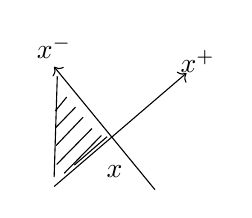
\begin{tikzpicture}[scale=0.8]
\draw[->] (-1.0,-0.8)--(1.1,1.0);
\draw[->] (0.6,-0.85)--(-1.0,1.1);
\draw (-1.0,-0.65)--(-0.95,0.95);
\draw (-0.96,-0.45)--(-0.40,0.12);
\draw (-0.97,-0.15)--(-0.54,0.30);
\draw (-0.98,0.13)--(-0.66,0.46);
\draw (-0.98,0.40)--(-0.80,0.62);
\draw (-0.84,-0.59)--(-0.25,0.01);
\draw (-0.68,-0.46)--(-0.16,-0.01);
\node at (-1.0,1.4) {$x^-$};
\node at (1.28,1.18) {$x^+$};
\node at (-0.04,-0.56) {$x$};
\end{tikzpicture}
\end{adjustbox}
\end{center}
\begin{equation*}
\text{(8)}_2\qquad
W_x^-=\{\ldots\mid w=0\text{ в заштр. обл.}\}.
\end{equation*}
[Внутри правой части фигурной скобки:]
\begin{center}
\begin{adjustbox}{max width=\linewidth}
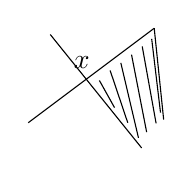
\begin{tikzpicture}[scale=0.8]
\draw (-1.0,-0.6)--(1.0,0.9);
\draw (-0.65,0.8)--(0.8,-1.0);
\draw (1.0,0.9)--(1.15,-0.55);
\draw (0.13,0.07)--(0.37,-0.36);
\draw (0.30,0.23)--(0.58,-0.60);
\draw (0.47,0.35)--(0.75,-0.84);
\draw (0.64,0.48)--(0.88,-0.75);
\draw (0.81,0.61)--(1.03,-0.61);
\draw (0.96,0.73)--(1.10,-0.44);
\node at (-0.15,0.36) {$x$};
\end{tikzpicture}
\end{adjustbox}
\end{center}

Если бы не ферми, а бозе, то ф-и --- аналог лагранжева разложения
на $p$ и $q$ (на 2 лагр. плоскости).

$A(W)$ --- [зачеркнуто: \Unclear{GELFAND-P000764}{clifford-cancelled-word}{неразборчиво}]
Клиффордова алгебра над $W$
\begin{equation*}
\{\psi_\mu^\pm\}\quad\text{--- базисы в }W_x^\pm
\end{equation*}
Клифф. алг. порожд. ими с соот.
\begin{equation*}
\text{(9)}_1\qquad
\psi_\mu^+\psi_\nu^-+\psi_\nu^-\psi_\mu^+
\underset{\mathrm{def}}{=}[\psi_\mu^+,\psi_\nu^-]=\delta_{\mu\nu}
\end{equation*}
\begin{equation*}
\text{(9)}_2\qquad
[\psi_\mu^+,\psi_\nu^+]=[\psi_\mu^-,\psi_\nu^-]=0
\end{equation*}
\Unclear{GELFAND-P000764}{eq9-last-superscript}{Последний верхний знак над $\psi_\nu$ густо закрашен; в формуле условно передан минусом.}

\underline{Обозначение:}
\begin{equation*}
\underline{\underline{\psi_\mu^-=\psi_\mu}}
\end{equation*}

\underline{Соотношение:}
\begin{equation*}
\text{(10)}\qquad A(W)=\Lambda(W_x^+)\cdot\Lambda(W_x)
\end{equation*}
\Unclear{GELFAND-P000764}{eq10-second-factor}{В последнем множителе записано $\Lambda(W_x)$ без видимого верхнего знака.}

Базисы ортогональные отн. скал. произведения (4).

Есть отображение:
\begin{equation*}
\begin{aligned}
A(W)&\longrightarrow\Lambda W_x^+\wedge\Lambda W_x^-\qquad\text{изоморфизм}\\
\lambda\cdot\mu&\overset{N}{\longrightarrow}\lambda\wedge\mu
\end{aligned}
\end{equation*}
обратное отображение:
\begin{equation*}
:\varphi:\ \longleftarrow\ \varphi
\end{equation*}
(произведение Вика)

В бозе-случае это „символ оператора“.

\SourcePage{GELFAND-P000765}{63}
% Повторные просмотры исходного кадра:
% просмотр 765–767; 765-top: [100,10,1470,550) x3.
% просмотр 765–767; 765-eq11: [100,540,2270,800) x3.
% просмотр 765–767; 765-eq12-13: [110,815,2180,1345) x3.
% просмотр 765–767; 765-eq14: [10,1320,2270,1610) x3.
% просмотр 765–767; 765-eq15-16: [80,1510,1950,1910) x3.
% просмотр 765–767; 765-vacua: [65,1860,1480,2610) x3.
% просмотр 765–767; 765-lower: [70,2600,1850,3270) x3.
% просмотр 765–767; 765-cancel11: [1205,580,1705,690) x6.
% просмотр 765–767; 765-cancel14: [265,1470,785,1570) x6.
% просмотр 765–767; 765-cancel15: [445,1538,575,1645) x10.
% просмотр 765–767; 765-cancel2: [525,1850,770,1940) x10.
% просмотр 765–767; 765-eq19-indices: [740,2700,1190,2825) x6.
% просмотр 765–767; 765-lastindex: [340,3070,465,3170) x10.
\underline{Определение.}
\begin{equation*}
\varphi_F(x)\in A(W)
\end{equation*}
\begin{equation*}
\operatorname{Spin}(W_x)=\{g\in A(W_x)\mid gW_xg^{-1}\subset W_x\}
\end{equation*}
На самом деле
\begin{equation*}
\varphi_F(x)\in\operatorname{Spin}(W)
\end{equation*}
Есть отображение:
\begin{equation*}
\operatorname{Spin}(W)\overset{T}{\longrightarrow}O(W);\qquad T_gw=gwg^{-1};
\tag{11}
\end{equation*}
[Между $O(W);$ и $T_gw$ зачёркнуто:
\Incomplete{GELFAND-P000765}{eq11-cancelled}{зачёркнутая фраза не читается полностью; различимо «а», далее знак, похожий на $T(g)$, и остатки букв}.
Над зачёркнутым вписано: «а именно:».]

$W$ имеет скал. произв. и, след., определено $O(W)$.
\begin{equation*}
T_{\varphi_F(x)}(w^++w^-)\underset{\mathrm{def}}{=}w^+-w^-
\tag{12}
\end{equation*}
(это определение $\varphi_F(x)$).

$T$ не мономорфно; поэтому пока некорр. опред. Точнее,
\begin{equation*}
\varphi_F(x)=:\exp L_F(x):
\tag{13}
\end{equation*}
где
\begin{equation*}
\begin{aligned}
\Lambda W\ni L_F(x)={}&\frac12\int_{-\infty}^{\infty}\int_{-\infty}^{\infty}
\underline{du}\,\underline{du'}\,\frac{-i(u-u')}{u+u'-i0}\cdot
\Psi(u)\Psi(u')\exp\biggl(-im\biggl(x^-(u+u')+{}\\
&{}+x^+\biggl(\frac1u+\frac1{u'}\biggr)\biggr)\biggr).
\end{aligned}
\tag{14}
\end{equation*}
[Под левой частью (14) зачёркнуто:
\Incomplete{GELFAND-P000765}{eq14-cancelled-words}{два зачёркнутых слова; возможное чтение «Можно говорить» не установлено}.]
Далее,

[Слева над (15) зачёркнут знак:
\Unclear{GELFAND-P000765}{eq15-cancelled-symbol}{неразборчивый зачёркнутый знак}.]
\begin{equation*}
\varphi^F(x)=\Psi_0(x)\exp L_F(x);
\tag{15}
\end{equation*}
где
\begin{equation*}
W\ni\Psi_0(x)=\int_{-\infty}^{\infty}\underline{du}\,\Psi(u)
\exp\biggl(-im\biggl(x^-u+\frac{x^+}{u}\biggr)\biggr)
\tag{16}
\end{equation*}
Есть [зачёркнуто:
\Incomplete{GELFAND-P000765}{vacuum-cancelled-word}{слово закрыто густой зачёркивающей линией; возможное чтение «векторы» не установлено}]
2 объекта:
\begin{equation*}
\langle vac|,\qquad |vac\rangle
\end{equation*}
\begin{equation*}
A(W)/A(W)W_x^-=|vac\rangle
\tag*{(17)$_1$}
\end{equation*}
\begin{equation*}
W_x^+A(W)\backslash A(W)=\langle vac|
\tag*{(17)$_2$}
\end{equation*}
Свойства:
\begin{equation*}
W_x^-|vac\rangle=0,\qquad\langle vac|W_x^+=0
\tag{18}
\end{equation*}
(естественные для вакуума).

Рассмотрим функцию
\begin{equation*}
\langle vac|\Psi(x_1)\ldots
\Psi(x_k)
\varphi_F(a_1)\ldots\varphi_F(a_m)|vac\rangle;
\tag{19}
\end{equation*}
($\Psi(x)$ из формулы (6)).

определенную на $(\mathbb R^2)^k$

Все $a_\nu$ фиксированы.

(2-мерн. модель Изинга ?)

\SourcePage{GELFAND-P000766}{unlabelled}
% Повторные просмотры исходного кадра:
% просмотр 765–767; 766-top: [65,0,2160,400) x3.
% просмотр 765–767; 766-eq21-22: [90,400,1680,735) x3.
% просмотр 765–767; 766-mid: [80,740,2040,1600) x3.
% просмотр 765–767; 766-eq24-notes: [90,1580,2230,2310) x3.
% просмотр 765–767; 766-eqa: [145,2280,2416,2520) x3.
% просмотр 765–767; 766-eqb: [115,2510,2416,2920) x3.
% просмотр 765–767; 766-bottom: [190,2910,2150,3320) x3.
% просмотр 765–767; 766-eq23-symbol: [390,1060,485,1150) x10.
% просмотр 765–767; 766-vectorindex: [1040,1260,1150,1380) x10.
% просмотр 765–767; 766-eqb-sign: [1650,2560,1760,2670) x10.
% просмотр 765–767; 766-bottomline: [350,2835,1530,2990) x3.
% просмотр 765–767; 766-matword: [595,2980,845,3090) x6.
\underline{\underline{$k=1$}} $\Rightarrow$
\begin{equation*}
\langle vac|\Psi(x)\varphi_F(a_1)\cdot\varphi^F(a_i)\ldots\varphi_F(a_n)|vac\rangle
\underset{\mathrm{def}}{=}W^i_{F,n}(x)
\tag{20}
\end{equation*}
[Подчёркивание волнистое:] \underline{Получается система ур-й}; положим
\begin{equation*}
M_F=z\partial_z-\bar z\partial_{\bar z}+\frac12
\begin{pmatrix}1&0\\0&-1\end{pmatrix}
\tag{21}
\end{equation*}
1-е ур-е имеет вид:
\begin{equation*}
M_Fw=(Bm^{-1}\partial_z-\bar Bm^{-1}\partial_{\bar z}+E)w
\tag{22}
\end{equation*}
\begin{equation*}
z=(x^0+x^1),\qquad\bar z=(x^0-x^1)
\end{equation*}
$B,E$ — пост. матрицы

2-е ур-е
\begin{equation*}
(m-\Gamma)w=0,\qquad\Gamma=\begin{pmatrix}0&1\\1&0\end{pmatrix}
\tag{23}
\end{equation*}
[\Unclear{GELFAND-P000766}{eq23-scalar-m}{В (23) буквально $m$; возможная ошибка источника или неуказанное соглашение}.]
\begin{equation*}
w_i=\begin{pmatrix}w_{i+}\\w_{i-}\end{pmatrix},\qquad
\begin{pmatrix}w_1\\w_n\end{pmatrix}
\end{equation*}
(22)--(23) — система максимально переопред.

(на самом деле это связность Гаусса-Манина).

Рассмотрим ещё
\begin{equation*}
\langle vac|\varphi_F(a_1)\ldots\varphi_F(a_n)|vac\rangle=\tau
\tag{24}
\end{equation*}
как функцию от $a$. ($\tau$-ф-я)

При $n=2$ это ф-я Пенлеве 3-го рода.

[Под «Пенлеве» вписано и подчёркнуто:] \underline{(Painleve)}

[Подчёркивание под именами волнистое:] \underline{Wu, Mc Coy, Tracy}, Phys. Rev. B13 (1976)

[Мелко под фамилиями:] что-то о ф-ях Пенлеве.

\underline{\underline{И.М.Г.}}

[«Garnier» подчёркнуто волнистой линией.]
Garnier — мемуар о ф-ях Пенлеве.

6 типов ур-й; 2-й пор.; особые точки неподвижные; самая общая
\begin{equation*}
\begin{aligned}
\frac1y y''={}&\frac a{x^2}+\frac b{(x-1)^2}+\frac c{(x-t)^2}
+\frac d{x(x-1)}+\frac3{4(x-\lambda)^2}\\
&{}+\frac\alpha{x(x-1)(x-t)}+\frac\beta{x(x-1)(x-\lambda)}
\end{aligned}
\tag{А}
\end{equation*}
Периоды (монодр.) не зависят от параметров $\Leftrightarrow$
\begin{equation*}
\begin{aligned}
\Leftrightarrow\quad\lambda''={}&\frac12\biggl(\frac1\lambda+\frac1{\lambda-1}+\frac1{\lambda-t}\biggr)\lambda'^2\\
&{}-\biggl(\frac1t+\frac1{t-1}
\text{\Unclear{GELFAND-P000766}{eqb-overwritten-sign}{неразборчивый исправленный знак}}
\frac1{t-\lambda}\biggr)\lambda'+{}\\
&{}+2\frac{\lambda(\lambda-1)(\lambda-t)}{t^2(t-1)^2}
\biggl[a+b+c+d+1-\biggl(a+\frac14\biggr)\frac t{\lambda^2}\\
&\qquad{}+\biggl(b+\frac14\biggr)\frac{t-1}{(\lambda-1)^2}
-\frac{ct(t-1)}{(\lambda-t)^2}\biggr]
\end{aligned}
\tag{Б}
\end{equation*}
У них одних — неподв. особые точки.

Постоянство матр. монодромии (А) $\Leftrightarrow$ неподв. особых точек (Б)

$t$, $\lambda$ меняются соглас. с (Б)

\SourcePage{GELFAND-P000767}{unlabelled}
% Повторные просмотры исходного кадра:
% просмотр 765–767; 767-header: [175,2780,2320,3200) x3.
% просмотр 765–767; 767-foot: [180,3170,2330,3472) x3.
[Верхняя большая часть кадра не содержит рукописного текста.]

\underline{$13/\overline{\underline{\mathrm{III}}}-78$}\qquad\underline{Сем. Гельфанда}

[Имя обведено красной прямоугольной рамкой и дважды подчёркнуто:]
\underline{\underline{Аомото}}.

\underline{Об обобщ. классич. гипергеом. ф-и с пом. интегралов}

\underline{типа}\quad\underline{Бернштейна} (И.)

[Ниже две текстовые области разделены двойной вертикальной чертой.]

[Слева, волнистое подчёркивание:] Ф-я Аппеля.

Случай 2-х перем.

[Справа:] И.М.Г.

[Волнистое подчёркивание:] Классич. гипергеом. ф-я.
\begin{equation*}
\sum_{n=0}^{\infty}x^n
\frac{\alpha(\alpha+1)\ldots(\alpha+n-1)\,\beta(\beta+1)\ldots(\beta+n-1)}
{\gamma(\gamma+1)\ldots(\gamma+n-1)\,n!}
\end{equation*}

\SourcePage{GELFAND-P000768}{unlabelled}
% Original inspected at 2416 x 3472. Review rectangles are source pixels,
% origin at upper left, format (x0,y0,x1,y1); enlargement does not add pixels.
% Full-page review includes both outer margins and the lower cancelled mark.
% Formula review: (485,65,1305,280) x4; (365,1290,1080,1435) x4;
% (500,1515,1320,1715) x4; (425,1930,1550,2190) x3.
\begin{equation*}
(1)\qquad F_1=\sum_{m,n\geq 0}
\frac{(\alpha,m+n)(\beta,m)(\beta',n)}
{(\gamma,m+n)(1,m)(1,n)}x^m y^n
\end{equation*}

\begin{center}—\quad$\cdot$\quad—\end{center}

\underline{И.М.Г.}\quad
\underline{\Unclear{GELFAND-P000768}{upper-heading}{Од.?} опр.}
\quad\underline{гипергеом. ф-й.}

% (330,400,1480,705) x3: two vertical strokes link the two expressions.
\begin{equation*}
\begin{gathered}
\bigl((x^2-1)^n\bigr)^{(n)}\qquad\text{(полин. Лежандра)}\\
\Vert\\
\bigl[((x-1)(x+1))^n\bigr]^{(n)}
\end{gathered}
\end{equation*}

\underline{Обобщение:}
\begin{equation*}
\bigl[(x-1)^{\alpha-1}(x+1)^{\beta-1}\bigr]^{(\gamma)}
\end{equation*}

% (290,895,645,1000) x8: heading ends in the plural -ы.
Интегралы порядка $\alpha$.
% (300,1000,2090,1310) x3; (1570,1040,2065,1170) x5.
\begin{equation*}
I_\alpha f=\int_0^x\frac{(x-t)^{\alpha-1}}{(\alpha-1)!}f(t)\,dt,
\qquad D^\alpha=I_{-\alpha}\quad\text{(аналитич. прод.)}
\end{equation*}
[Под знаменателем $(\alpha-1)!$ скобкой подписано $\Gamma(\alpha)$.]

\begin{equation*}
\bigl[x^{\alpha-1}(1-x)^{\beta-1}\bigr]^{(\gamma)}
\end{equation*}

% Properties inspected at x3 and individually at x5/x6:
% (870,1430,1410,1525); (1470,1430,1975,1525); (1990,1430,2290,1550).
Гипергеом. ф-я: 1) хор. разл. в ряды\quad
2) хорошее дифф. ур-е\quad
3) хороший интегр см.

\begin{equation*}
\int_0^x t^{\alpha-1}(1-t)^{\beta-1}(x-t)^{\gamma-1}\,dt
\end{equation*}

$B$-ф-и проще.

\begin{center}—\quad$\cdot$\quad—\end{center}

\begin{equation*}
(\alpha,n)=\alpha(\alpha+1)\ldots(\alpha+n-1)
\end{equation*}

\begin{equation*}
(2)\qquad F_4=\sum_{m,n\geq 0}
\frac{(\alpha,m+n)(\beta,m+n)}
{(\gamma,m)(\gamma',n)(1,m)(1,n)}
\end{equation*}
\Unclear{GELFAND-P000768}{series-f4}{В записи (2) множитель $x^m y^n$ не виден.}

Имеется интегральное представление
[зачёркнуто: \Unclear{GELFAND-P000768}{lower-heading-cancellation}{неразборчивый знак}]
для $F_1$

(3)\quad
\SourceFigure{GELFAND-P000768}{diagram-01}{Четыре пересекающиеся прямые: почти вертикальная слева с подписью 1 снизу, круто наклонённая вправо вниз с подписью 2, полого наклонённая вправо вниз с подписью 3 и почти горизонтальная с подписью 4 справа. На правом конце последней короткий косой штрих; близкие верхние пересечения и значение этого штриха требуют проверки по оригиналу.}

\begin{equation*}
\int f_1^{\lambda_1}f_2^{\lambda_2}f_3^{\lambda_3}f_4^{\lambda_4}\,da\,db
\end{equation*}
[В $db$ буква $b$ обведена или исправлена:
\Unclear{GELFAND-P000768}{integral-differential}{первоначальное начертание неразборчиво}.]

$f_j$ — лин. формы; $x,y$ сод. среди коэффициентов.

% (270,2760,2320,3220) x3; (1110,2850,1320,2970) x5.
3 прямые прив. к прост. виду (афф. преобр.) и фиксируются

4-я зад. параметрами $a,b$.

$F_2,F_3$ получ. аналогично, но с другим
[зачёркнуто: \Unclear{GELFAND-P000768}{lower-cancelled-word}{расп.?}]
расп. прямых, (не общего полож.):

[Слева внизу зачёркнуто:
\Unclear{GELFAND-P000768}{bottom-cancellation}{$F_1$?}.]

% Diagram inspected at source (660,3090,940,3370) x4.
% Two nearly horizontal and two nearly vertical strokes, plus a descending
% diagonal; the right vertical stroke begins on the diagonal. No labels.
\begin{center}
\begin{adjustbox}{max width=\linewidth}
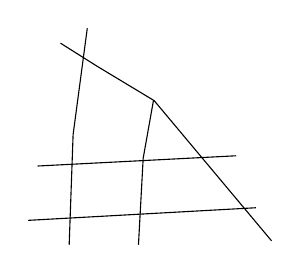
\begin{tikzpicture}[x=1cm,y=1cm]
\draw (0.55,0.05) -- (0.60,1.45) -- (0.78,2.80);
\draw (1.43,0.05) -- (1.49,1.15) -- (1.62,1.88);
\draw (0.03,0.36) -- (2.92,0.52);
\draw (0.15,1.05) -- (2.67,1.18);
\draw (0.44,2.61) -- (0.90,2.32) -- (1.63,1.88) -- (3.12,0.10);
\end{tikzpicture}
\end{adjustbox}
\end{center}

\SourcePage{GELFAND-P000769}{68}
% Full original inspected at original detail. Text/math crops at 3x;
% cancelled opening at (215,465,610,560), 5x; rank at
% (1675,2570,2000,2680), 10x; minor at (240,2625,1160,2830), 5x.

$F_4:$
\begin{adjustbox}{max width=\linewidth}
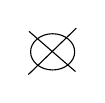
\begin{tikzpicture}[x=1cm,y=1cm,baseline=-0.2cm]
\draw (0,0) ellipse (0.28 and 0.23);
\draw (-0.31,-0.29) -- (0.30,0.30);
\draw (-0.30,0.26) -- (0.29,-0.25);
\end{tikzpicture}
\end{adjustbox}
вместо 2-х прямых берётся квадр. форма.

% The two following source lines are underlined with a wavy line.
\underline{Число лин. независ. реш. соотв. дифф. ур-й = числу огранич.}
\newline
\underline{связных компонент соотв. картины.}

\underline{Общее замеч. о коэфф.:} отношение соседних = рац. ф-я от $m,n$.

\Unclear{GELFAND-P000769}{cancelled-opening}{зачёркнуто, неразборчиво}
Аналогичную задачу можно делать с любым числом гиперплоскостей

$$
(4)\qquad f_i=\sum_{\nu=1}^{n}a_{i\nu}x_\nu+a_{i0}
$$
$$
1\le i\le m
$$
$$
f_{m+1}=1\qquad\text{Обычно }m\ge n.
$$
Рассмотрим матрицу из набора коэффициентов форм
$$
(5)\qquad
A=\begin{pmatrix}
a_{10}&\ldots&&a_{1n}\\
\vdots&&&\\
a_{m0}&\ldots&&a_{mn}\\
1&\ldots&0&0
\end{pmatrix}
\in\mathbb C^{m(n+1)}
$$
Там действует афф. группа от $n$ переменных
\newline
(на $x$ она действует)
\newline
— Замена переменного по $x$
% "по x" checked at (870,1520,1050,1635), 10x.

Пусть
$$
\mathcal M\subset\mathbb C^{m(n+1)}\times\mathbb C^n
$$
состоит из пар
$$
\{(A,x):f_j(x)\ne0\}\qquad\text{(не удовл. ни одно ур-е)}
$$
(дополн. ко всем гиперплоскостям)

\begin{center}
\begin{adjustbox}{max width=\linewidth}
\begin{tikzcd}
\mathbb C^{m(n+1)}\times\mathbb C^n\arrow[d,"\pi"]\\
\mathbb C^{m(n+1)}
\end{tikzcd}
\end{adjustbox}
\end{center}

$$\gamma\subset\mathcal M$$
м-во таких ур-й, что гиперпл. не в общем положении
\newline
\Unclear{GELFAND-P000769}{rank-correction}{\underline{ранг $\le n$}}

$$
[i_1\ldots i_{n+1}]=
\begin{vmatrix}
a_{i_1 0}&\ldots&a_{i_1 n}\\
\vdots&&\\
a_{i_n 0}&&i_n n
\end{vmatrix}
\qquad\text{(минор, получ. из строк }i_1,\ldots,i_n\text{)}
$$
\Unclear{GELFAND-P000769}{minor-indices}{в скобках $i_{n+1}$; в последней строке и пояснении $i_n$; нижний правый элемент $i_n n$}

% Crossed symbol reviewed at (270,2800,405,2920), 10x.
Проекция
\Unclear{GELFAND-P000769}{projection-cancelled-symbol}{зачёркнутый знак, возможно $\gamma$}
$\gamma$ зад. усл. на миноры:
$$
(6)\qquad Y=\{A\mid[i_1,\ldots,i_{n+1}]=0\}
\qquad
\begin{adjustbox}{max width=\linewidth}
\begin{tikzcd}
\gamma\arrow[d,"\pi"]\\
Y
\end{tikzcd}
\end{adjustbox}
$$
% The separate overwritten mark is below the equation at left, not a new relation.
% Reviewed in (210,3030,425,3190), 10x, and full original.
\Unclear{GELFAND-P000769}{bottom-cancelled-symbol}{отдельный обведённый знак, возможно $\gamma$}

\SourcePage{GELFAND-P000770}{unlabelled}
% Full original inspected at original detail. Dense text/formulas viewed at 3x.
% Bottom cohomology identity reviewed at (325,3090,2395,3435), 3x;
% chi glyph additionally at (830,3110,1060,3270), 10x.

% The source's vertical leader goes from S_A to its explanation below.
\begin{center}
\begin{adjustbox}{max width=\linewidth}
\begin{tikzpicture}[x=1cm,y=1cm]
\node at (0,0) {$\pi^{-1}(A)\cong\mathbb C^n\setminus$};
\node (s) at (2.15,0) {$S_A$};
\node at (5.1,0) {$,\qquad A\in X\setminus Y$};
\node (t) at (2.15,-0.95) {объед. $m$ гиперпл. общего положения};
\draw (s.south) -- (t.north);
\end{tikzpicture}
\end{adjustbox}
\end{center}

$\Omega_A^{\bullet}$ — комплекс рац. форм в $\mathbb C^n$ с полюсами на $S_A$
\newline
(внешнее диффер.)

$\forall\varphi\in\Omega_A$ есть ф-ла
$$
U=f_1^{\lambda_1}\ldots f_m^{\lambda_m},
$$
$$
d_x(U\varphi)=U\underbrace{(\omega\wedge\varphi+d_x\varphi)}_{=\nabla_\omega\varphi},
$$
% The manuscript's brace and diagonal equality leader identify nabla_omega phi.
Здесь
$$
\omega=\sum_{1}^{m}\lambda_j\frac{df_j}{f_j}
\qquad (\nabla_\omega\text{ — связность}).
$$
$\omega$ — форма связности
$$
\nabla_\omega:\Omega_A^p\longrightarrow\Omega_A^{p+1}
$$
$$
\nabla_\omega\varphi=\omega\wedge\varphi+d_x\varphi
$$
(связность в тривиальном расслоении)

Имеем:
$$d\omega+\omega\wedge\omega=0$$
(усл. интегрируемости)

Отсюда вытекает, что $\nabla_\omega^2=0$ и мы получаем комплекс.

\underline{Делинь, Гротендик:} возник. теория рац. гиперкогомологий де Рама.

\underline{Предположение.}
$$\lambda_{m+1}=-\lambda_1-\ldots-\lambda_m$$
$\forall$ наб.
$$
1\le i_1<\ldots<i_\nu\le m+1,\qquad1\le\nu\le n.
$$
\underline{Условие:}
$$
\lambda_{i_1}+\ldots+\lambda_{i_\nu}\notin\mathbb Z^+
\qquad
\mathbb Z^+=\{n\in\mathbb Z,\ n>0\}
$$

\underline{Предл.}
$$
H^p(\Omega_A,\nabla_\omega)=0,\quad p\ne n
$$
$$
H^n(\Omega_A,\nabla_\omega)=\chi(\mathbb C^n\setminus S_A)\cong
\frac{
\underset{\substack{=\ \mathrm{def}\\\Omega^n(\log\langle S\rangle)}}{
\left\{\frac{df_{i_1}}{f_{i_1}}\wedge\ldots\wedge\frac{df_{i_n}}{f_{i_n}}\right\}}
}{\omega\wedge\Omega^{n-1}(\log\langle S\rangle)}
$$
% Source definition is written below the numerator with a vertical equality
% and "def" at its side; it is kept below the displayed generating forms.
\Unclear{GELFAND-P000770}{cohomology-euler}{$H^n(\Omega_A,\nabla_\omega)=\chi(\mathbb C^n\setminus S_A)$, без видимого $\dim$}

\SourcePage{GELFAND-P000771}{69}
% Full original inspected at original detail. All text/formulas viewed at 3x.
% Inserted qualifier reviewed at (1355,756,1670,855), 8x.

\underline{Пояснение:}
$$
\Omega^1(\log\langle S\rangle)=\left\{\frac{df_i}{f_i}\right\}_{i\le m}
$$
$$
\bigwedge\Omega^1(\log\langle S\rangle)/\sim\ =\Omega^{\bullet}(\log\langle S\rangle)
$$
\begin{center}
\begin{adjustbox}{max width=\linewidth}
\begin{tikzcd}[column sep=small]
0\arrow[r]&\mathbb C\arrow[r,"\omega\wedge"]&\Lambda^1\arrow[r,"\omega\wedge"]&\cdots\arrow[r,"\omega\wedge"]&\Lambda^n\arrow[r]&0
\end{tikzcd}
\end{adjustbox}
\end{center}

(Они замкнуты: $\nabla_\omega=\omega\wedge$ для таких форм)

$$
\chi(\mathbb C^n\setminus S_A)=\binom{m-1}{n}=
\text{число (относит.) компактных связных}
$$
компонент $\mathbb R^n\setminus S_A$
% "(относит.)" is an above-line insertion before "компактных".

\begin{center}— , —\end{center}

$$\int U\varphi$$
% These are side-by-side in the source: integral at left, the cancellation
% and heading "Двойственность" at right; phi membership is under the integral.
\Unclear{GELFAND-P000771}{cancelled-duality}{зачёркнуто, неразборчиво}
Двойственность
\newline
$\varphi\in\Omega_A$

$U$ многозначна $\Rightarrow$ при обходе получаем предс. фунд. группы:
$$
\ell_U:\pi_1(\mathbb C^n-S_A)\longrightarrow\mathbb C^*
$$
(при обходе умн. на ненулевое компл. число)

Пусть взята соотв. лок. система
$$
\zeta_\ell\text{ — лок. система,}\qquad\zeta_\ell^*\text{ — дуальная.}
$$
% Tentative glyph zeta is repeated consistently, not silently resolved.
% Introductory symbols: (320,1640,1670,1800), 4x;
% starred symbol: (1125,1660,1250,1810), 10x.
\Unclear{GELFAND-P000771}{local-system-symbol}{знак лок. системы: возможно $\zeta_\ell$, $\mathcal L_\ell$ или $\xi_\ell$}

Есть двойств.
$$
H^n(\mathbb C^n\setminus S_A,\zeta_\ell)\times
H_n(\mathbb C^n-S_A,\zeta_\ell^*)\longrightarrow\mathbb C
$$

$\forall$ комп. связной компоненте $\longrightarrow$ эл $\in$
$H_n(\mathbb C^n-S_A,\zeta_\ell)$
% Last coefficient is strongly overwritten; reviewed at
% (1700,1950,1835,2100), 10x; no unambiguous star is visible.
\Unclear{GELFAND-P000771}{component-coefficient}{сильно обведённый знак лок. системы с индексом $\ell$; звёздочка неразличима}

\SourcePage{GELFAND-P000772}{unlabelled}
% Review: original 2416 x 3472 inspected; upper portion blank. Heading crop [230,1540,1940,1860], 3x.
\underline{\underline{20/III-78 г.}} \qquad \underline{Сем. Гельфанда}

\begin{adjustbox}{max width=\linewidth}
\begin{tikzpicture}[baseline=(speaker.base)]
\node[draw=red,rectangle,inner sep=4pt] (speaker) {В. М. Бухштабер.};
\draw ([yshift=-2pt]speaker.south west) -- ([yshift=-2pt]speaker.south east);
\end{tikzpicture}
\end{adjustbox}
\quad (+ А. В. Шокуров)
% The scan has a red rectangular frame around the name and a black underline below it.
% Review: co-speaker surname [955,1650,1173,1737], 10x; visible initials retained as А. В.

\underline{Алгебры Ландвебера-Новикова и форм. вект. полей на прямой.}
% Review: cancellation below title, [570,1800,660,1860], 10x.
\Unclear{GELFAND-P000772}{title-cancellation}{Зачёркнуто: неразборчиво.}

$\mathbb R^1$, $\operatorname{Diff}_1$ — форм. диффеом. прямой с доп. условием: $\varphi'(0)=1$
$$
\varphi(0)=0,\qquad \varphi'(0)=1
$$

Группа $=\underset{\longleftarrow}{\lim}$ конечномерных групп

(в струях пор. $n$)

Алг. Ли — алг. Ли форм. вект. полей на $\mathbb R^1$ — это $L_1$.
$$
t+a_1t^2+\ldots+a_nt^{n+1}+\ldots
$$
$a_j$ — координаты.

Кольцо функций: $\underline P$ (полиномы от всех $a_j$).

\underline{Род Хирцебруха:} $M$ — компл. или стаб. комплексное мн-ие

% Review: cancellation preceding M, [376,2680,466,2792], 10x.
\Unclear{GELFAND-P000772}{genus-cancellation}{Зачёркнуто: неразборчиво.}
$M\rightsquigarrow M(\varphi)$ — полином на $\operatorname{Diff}_1$.
$$
\frac{t}{\varphi(t)}=\psi(t)
$$
$$
\prod_{j=1}^{N}\psi(\beta_jt),\qquad N>\dim_{\mathbb C}M
$$

Коэффициент при $t^n$ = симметрическая ф-я от $\beta_j$ =

$=\Omega(\sigma_1,\ldots,\sigma_N)$, $\sigma_j$ — элем. симм. полиномы

\SourcePage{GELFAND-P000773}{75}
% Review: full original 2416 x 3472 inspected, including visible top-right 75; successive 3x crops cover all writing.
$\sigma_j\rightsquigarrow j$-й класс Черна

Рассмотрим
$$
\langle\Omega(\sigma_1,\ldots,\sigma_N),M\rangle
$$
это и есть ф-я на $\operatorname{Diff}_1$.

% Review: top-left cancelled text [331,379,539,474], 8x.
\Unclear{GELFAND-P000773}{top-cancellation}{Зачёркнуто: неразборчиво.}
Операции над мн-иями $\rightsquigarrow$ операции над полиномами.

левоинв. дифф.-операторы — ?

1) $M\times M_1$

2)
$\begin{adjustbox}{max width=\linewidth}
\begin{tikzcd}[row sep=small]
\tau\arrow[d]\\
M
\end{tikzcd}
\end{adjustbox}$
— кан. рассл.

$c_1(\tau)\rightsquigarrow$ двойств. ему цикл $M_1\subset M$

$\operatorname{Codim}_{\mathbb C}M_1=1$.

(нули сечений кан. расслоения).

Аналог: двойств. к $\forall$ полиному от классов Черна.

Ландвебер-Новиков; ничего другого нет. (это все естеств. когомологич. операции)

\underline{Теорема 1.}

% Review: two parallel downward arrows only; no horizontal arrows visible, [240,1140,1840,1795], 3x.
$$
\begin{adjustbox}{max width=\linewidth}
\begin{tikzcd}
M\arrow[d,"c_\omega"] & M(\varphi)\arrow[d]\\
M_\omega & D_\omega M(\varphi)
\end{tikzcd}
\end{adjustbox}
$$

$c_\omega$ — полином от кл. Черна

$D_\omega$ — левоинв. дифф. оператор.

$\Longleftrightarrow$ вз. однозн. соответствие

$M(\varphi)$ — целочисл. полиномы

Когда полиномы отвечают мн-ям?

\underline{Ответ:}

\underline{\underline{Теор. 2.}}

$\operatorname{Diff}_1(\mathbb Z)$ — форм. дифф. с целочисл. коорд.

Род Тодда $\varphi=\underline{1-\exp(-t)}$ (диффеоморфизм)

\underline{Полином должен принимать целые знач. на правом}

\underline{смежном классе этого $\varphi$}
% Review: overdrawn letter between phi and Diff [1094,2293,1200,2388], 8x.
\Unclear{GELFAND-P000773}{todd-cancellation}{Зачёркнуто: в?}
$\underline{\operatorname{Diff}_1(\mathbb Z)}$.

% Review: isolated cancelled mark [390,2390,469,2498], 8x.
\Unclear{GELFAND-P000773}{stong-cancellation}{Зачёркнуто: неразборчиво.}
($\sim$ теор. \underline{Стонга-Хаттори})

$S$ — мн-во всех опер. Ландвебера-Новикова; это алгебра.

Сложение: несвязное объединение, умн. — композиция.

\underline{Когомологии этой алг.} важны. Через них выраж. все

гомотопич. инвар. непр. отобр. (Новиков)

\underline{Теор. 3}
$$
\operatorname{Ext}_S(\mathbb Q,\mathbb Q)=H^*(L_1)
$$

% Review: abbreviated word after equality [350,3050,1600,3187], 5x, and [950,3075,1120,3170], 10x.
Когом. алгебра = когом обёрт. алг.

$H^*(L_1)$ посчитано в раб. Гельф., Фукса, Гончаровой

\underline{Задача:} посчитать когомологии группы $\operatorname{Diff}_1(\mathbb Z)$.

\SourcePage{GELFAND-P000774}{unlabelled}
% Additional final review: «Шредингером» (600,260,1160,360), 6x;
% equation (1) (255,395,1390,505), 4x.
% Original inspected in full at 2416 x 3472 pixels. Enlarged review regions:
% heading (250,60,2170,355), 3x; operator/note (340,490,1890,775), 3x;
% Fourier (400,765,1380,1300), 3x; right margin (1430,800,2390,1180), 3x;
% middle (300,1300,2210,1930), 3x; scattering (300,1900,2320,2580), 3x;
% bottom (260,2550,2250,3310), 3x; spectral symbol (850,2070,1340,2230), 8x;
% equation (4') (430,2470,1300,2610), 6x.
\underline{\underline{Калоджеро.}} (и A. De gasperis).

Класс нелин. эволюц. ур-й, решаемых с пом. спектр. преобр.,
ассоц. \textbf{с} Шредингером.
% The preposition after «ассоц.» is heavily retraced in the source.

\begin{equation}
u_t(x,t)=\alpha(\underline{L},t)u_x(x,t) \tag{1}
\end{equation}
\begin{equation}
\underline{L}f(x)=f_{xx}-4u(x,t)f(x)
 +2u_x(x,t)\int_x^{\infty}dx'\,f(x') \tag{2}
\end{equation}
% «лин.» is above the prose; the insertion mark points between «Реш.» and «зад.».
Реш. [Над строкой, со знаком вставки: лин.] зад. Коши свод. к лин. задаче для пр. Фурье

$$
u(x,t)\underset{\text{Фурье}}{\Longleftrightarrow}u(k,t)
$$
$$
u_t(x,t)=-i\omega\left(-i\frac{\partial}{\partial x},t\right)u(x,t)
$$
$$
\hat{u}_t(k,t)=-i\omega(k)\hat{u}(k,t)
$$
\Unclear{GELFAND-P000774}{fourier-notation}{Справа в первой строке $u(k,t)$ без видимой шляпки; в последней строке $\omega(k)$ без аргумента $t$.}

% Right-margin note, separated from the main column by two vertical strokes.
\begin{quote}
Более шир. класс:
$$
\left\Vert\begin{aligned}
u_t&=\cdots-ix\omega'(\ldots)\\
\hat{u}_t&=\cdots\quad\cdots\frac{\partial\hat{u}}{\partial k}
\end{aligned}\right.
$$
\end{quote}

можно реш. более шир. класс. ур-й:
\begin{equation}
u_t(x,t)=\alpha(\underline{L},t)u_x(x,t)
 +\beta(\underline{L},t)[xu_x(x,t)+2u(x,t)] \tag{3}
\end{equation}

$\alpha$ --- ф-я от оператора

$\beta$ --- тоже

$$
\alpha(\underline{L},t)=-\underline{L}\quad\Rightarrow\quad
 KdV\quad(\text{при }\beta=0)
$$
Здесь есть и высшие KdV: $\alpha(z,t)=z^k$.

Для (3) есть линейная спектр. задача, опис. эволюцию $u$.
$$
u(x,t)\Longleftrightarrow\{R(k,t);p_n,c_n^2\}
$$
\Unclear{GELFAND-P000774}{spectral-letter}{$p_n$ или $\rho_n$; тот же знак в (4').}
(реш. ур-я Гельф. --- Левитана)

\begin{equation}
R_t(k,t)=2ik\alpha(-4k^2,t)R(k,t)-k\beta(-4k^2,t)R_k(k,t) \tag{4}
\end{equation}
\begin{equation}
p_t(t)=p(t)\beta(-4p^2,t) \tag{4'}
\end{equation}

для $c$ ур-е как для $R$ (не выписывается)

Скорость солитонов не сохраняется и амплитуда тоже.

\underline{Законы сохранения.}
\begin{equation}
c^{(n)}=\int_{-\infty}^{\infty}dx\,\underline{L}^{n}[xu_x(x,t)+2u(x,t)] \tag{5}
\end{equation}

\underline{Теорема 1.} $\beta\equiv0\quad\Rightarrow\quad(c^{(n)})_t=0$

(в частности: KdV).

\SourcePage{GELFAND-P000775}{76}
% Additional final review: Schrödinger/wave region (110,1690,1490,2210), 3x;
% visible page label (2190,35,2370,150), 6x.
% Original inspected in full at 2416 x 3472 pixels. Enlarged review regions:
% top (145,30,1660,735), 3x; operators (455,760,1760,1190), 3x;
% recurrence (80,1220,2310,1690), 3x and (535,1470,1140,1680), 6x;
% phase formulas (300,2140,1920,3030), 3x.
AKNS

(Ablowitz, Kaup, Newell, ---)

--- такая запись высших KdV.

Для 2-х гам. структур запис. KdV.

Скобок Пуасс. --- беск. число.

Запись высш. KdV с \underline{интегралом}: $\displaystyle\int_{-\infty}^{\infty}u^2dx$.

(Фаддеев и др. --- ленинградцы)

\underline{и сложной гам. структ.}
% This last underline is wavy in the source.

$$
I_0=\int u^2dx;\qquad
\underline{\underline{u_t=A_n\frac{\delta I_0}{\delta u(x)}}};
\qquad\text{это высш. KdV}
$$
$$
\underline{\underline{A_n=\underline{L}^{n}\frac{\partial}{\partial x}}}
$$
% Both emphasized formulas have broad bracket-like double underlining;
% the lower strip beneath A_n contains short hatch strokes.

Законы преобр. инв. относит. сдвига по $x$, а в интеграл входит $x$.

% «Новиков:» is written in the left margin and has a wavy underline.
\underline{Новиков:}
$$
L_3c_n=\frac{\partial}{\partial x}c_{n+1}
\quad\Rightarrow\quad
\left[\left(\frac{\partial}{\partial x}\right)^{-1}L_3\right]c_n=c_{n+1}
$$
$\Rightarrow$ возник. степени опер.
$$
\underline{L}=\partial^{-1}L_3
$$
\Unclear{GELFAND-P000775}{operator-order}{В исходнике $\underline{L}=\partial^{-1}L_3$; порядок множителей сохранён.}

Рассм. ур-е Шред.
\begin{equation}
\Psi_{xx}=[u(x)-k^2]\Psi \tag{6}
\end{equation}
$$
\Psi(k,x)\underset{x\to-\infty}{\longrightarrow}T(k)e^{-ikx}
$$
$$
\Psi(k,x)\underset{x\to+\infty}{\longrightarrow}e^{-ikx}+R(k)e^{ikx}
$$
$$
T(k)=|T(k)|e^{2i\varphi(k)}
$$
$$
T(\pm k)=|T(k)|e^{\pm2i\varphi(k)}
$$
\begin{equation}
\varphi(k)=\sum_{n=0}^{N}k^{-(2n+1)}\varphi^{(n)}+O(k^{-(2N+3)}). \tag{7}
\end{equation}

Тогда
\begin{equation}
\fbox{$\displaystyle\varphi^{(n)}=(-1)^{n+1}[2(2n+1)]^{-1}c^{(n)}$} \tag{8}
\end{equation}
\begin{equation}
u_t(x,t)=\alpha(\underline{L},t)u_x(x,t)
+\beta(\underline{L},t)[xu_x(x,t)+2u(x,t)] \tag{9}
\end{equation}

\SourcePage{GELFAND-P000776}{unlabelled}
% Additional final review: calligraphic L (370,2580,730,2700), 8x.
% Original inspected in full at 2416 x 3472 pixels. Enlarged review regions:
% top (155,20,1780,840), 3x; integral glyphs (360,200,1480,390), 4x;
% heading (190,850,1920,1110), 3x; date (220,875,535,990), 8x;
% middle prose (220,1380,2380,2100), 3x; «жгучая» (700,1410,1020,1530), 8x;
% mirror-left (295,1110,845,1400), 3x; mirror-right (1065,1150,1670,1390), 3x;
% dynamic drawing (325,1720,560,2000), 5x; surface (245,2110,520,2470), 5x;
% bottom (175,2480,2325,3420), 3x; final data (1270,3030,2160,3360), 4x.
Пусть
\begin{equation}
\beta(z,t)=\sum\beta_n(t)z^n \tag{10}
\end{equation}
Тогда получ. беск. система:
\begin{equation}
C_t^{(n)}(t)=n\sum_m\beta_m(t)c^{(n+m)}(t) \tag{11}
\end{equation}
\Unclear{GELFAND-P000776}{integral-case}{Регистр знака $C/c$ в (11): слева более крупный $C$, справа более мелкий $c$.}

$\beta$ --- полином по $z$ $\Rightarrow$ сист. треугольная.

$\beta_0=i\omega$ $\Rightarrow$ все величины периодич. по $t$.

(следствие структуры)

\underline{\underline{След. раз. --- о пр. Бэклунда}}
% The underline is heavily reinforced and hatched, below rather than through the words.

\bigskip
\underline{21/III-78.}\qquad\underline{В. П. Паламодов}\qquad\underline{на обществе.}

\underline{Лакуны, резкие фронты и деформации особенностей.}

\SourceFigure{GELFAND-P000776}{diagram-parabolic}{Слева рисунок с подписью «параболич. зеркало»: открытая вверх U-образная кривая; внутри несколько вертикальных отрезков, доходящих до разных точек нижней дуги, и наклонные отрезки, пересекающиеся выше дна. В месте их пересечения короткие перекрещённые штрихи. Наконечники стрелок не различимы.}

\SourceFigure{GELFAND-P000776}{diagram-spherical}{Справа рисунок с подписью «сферич. зеркало»: широкая U-образная кривая, три почти вертикальных внутренних отрезка к левой половине нижней дуги, наклонные отрезки к правой верхней области; поверх них две густо проведённые кривые сходятся в направленный вниз острый выступ. Места слияния линий не позволяют однозначно воспроизвести все соединения.}

Каустика --- «жгучая», «горячая» (по гречески)

Отраженные от сферич. зеркала лучи касаются кривой с особенн. ---

--- каустики.

Динамич. картина: волн. фронты

\SourceFigure{GELFAND-P000776}{diagram-wave-fronts}{Рисунок слева: две вложенные открытые вверх U-образные кривые; в их верхней и центральной области пересекающиеся наклонные, почти вертикальные и дугообразные штрихи, в том числе густо обведённые линии, сходящиеся в нижний острый конец внутри меньшей U-образной кривой. Несколько тонких ветвей продолжаются вверх. Отдельные пересечения и слияния неразличимы.}

в момент образования каустики особ. $\underline{\underline{y=x^{4/3}}}$

Есть поверхность, гориз. сеч. к-той совпадают с положениями фронта

\SourceFigure{GELFAND-P000776}{diagram-surface}{Рисунок под текстом: контур из нескольких изогнутых линий, образующий два расположенных один над другим широких раскрытия влево и узкую заострённую часть справа вверху. Слева видны почти вертикальные участки, один из них прерывистый. Справа три утолщённые точки расположены одна под другой на изогнутой линии; от верхней идут пересекающиеся ветви, от средней короткая дуга направо. Разрывы, пересечения и возможное перекрытие частей поверхности нельзя уверенно разграничить. Подписей нет.}

Рассмотрим гиперболическое ур-е
\begin{equation}
\mathcal{L}(x,D)u=0, \tag{1}
\end{equation}
например
\begin{equation}
\left(\frac{\partial^2}{\partial t^2}-\frac{1}{c^2}\Delta\right)u=0 \tag{2}
\end{equation}

Фундаментальное решение:
\begin{equation}
\mathcal{L}(x,D)E=0,\quad t>0,\qquad
\left.\frac{\partial^jE}{\partial t^j}\right|_{t=0}
 =\delta(x')\delta_{j,m-1},\qquad
j=0,1,\ldots,m-1 \tag{3}
\end{equation}

\end{document}
